\documentclass[nobiblatex]{LTHthesis}
\usepackage[T1]{fontenc}
\usepackage[utf8]{inputenc}
\usepackage{graphicx}
\usepackage{mathptmx, helvet}
\usepackage{xfrac}
\usepackage[left=2.5cm,right=2.5cm,top=3cm,bottom=5cm]{geometry}
\usepackage{listings}
\usepackage{color}
\usepackage{url}
\usepackage{verbatim}
\usepackage[]{algorithm2e}
\usepackage{lipsum}
\usepackage{titlesec}
\usepackage{todonotes}
\usepackage{framed}
\usepackage{nicefrac}
\usepackage{amsmath} % assumes amsmath package installed

\newsubfloat{figure}

\newcommand{\martina}[1]
  {\todo[inline,color=red!30,caption={}]{\textbf{Martina:} #1}}

\newcommand{\newstuff}[1]%
  {\todo[inline,color=green!30,caption={}]{\textbf{New stuff:} #1}}
  
\newcommand{\tv}{\tilde{v}}
\definecolor{red}{rgb}{1,0,0}

\newtheorem{proposition}{Proposition}[section]

\begin{document}


\lstset{
  language=C,
  basicstyle=\footnotesize,
  numbers=left,
  numberstyle=\footnotesize,
  stepnumber=1,
  numbersep=5pt,
  backgroundcolor=\color{white},
  showspaces=false,
  showstringspaces=false,
  showtabs=false,
  frame=leftline,
  tabsize=2,
  captionpos=b,
  breaklines=true,
  breakatwhitespace=false,
  escapeinside={\%*}{*)},
  xleftmargin=2\parindent,
  keywordstyle=\bfseries\color{green!40!black},
  commentstyle=\itshape\color{purple!90!black},
  identifierstyle=\color{black},
  stringstyle=\color{orange},
}

%\textcolor{red}{2do:}

\begin{verbatim}
\end{verbatim}





\begin{titlepages}
\author{Fredrik Johnsson and Olle Svensson}
\title{Resource management and prioritization in an embedded Linux system}
\year{2014}
\month{June}
\TFRT{9999}  %%  You will get the number from the department.
\printer{Media-Tryck} %% You may get other information from the department.

\end{titlepages}
\setcounter{page}{1}
\pagenumbering{roman}

\chapter*{Abstract}

This master thesis tackles the problem of limited computing resources on a
camera that is executing computing applications together with image
acquisition and streaming. The thesis was carried out at Axis Communications
in cooperation with the Department of Control at Lunds University. The
problem of limited resources on an Axis camera is handled by a two part
solution where a resource manager (RM) distributes the available resources
and services can adapt their service level (SL) in order to finish their
jobs on time. The solution is based on game theory, where services are
players, varying their service levels in order to get a good match between
given resources and their computing requirements. This service level
adaptation scheme is partially implemented for the streaming service on the
camera and for some test services, performing mathematical operations. The
resource manager is incorporated into \texttt{systemd}, and uses 
\texttt{cgroups}~\cite{cgroups} to distribute the computing capacity. The
experimental results show that the resource manager is fully operational and
capable of managing and prioritizing resources as intended on the embedded
system. However the work with adapting the video quality adaptation is still
left to be completed.

\chapter*{Acknowledgements}

We want to thank our supervisors, Umut Tezduyar-Lindskog, Axis and Martina 
Maggio, LTH Department of Control. We would also like to thank engineering 
manager Pontus Bergendahl, Axis.


\tableofcontents
\newpage

\setcounter{page}{1}
\pagenumbering{arabic}

\chapter{Introduction}

This master thesis treats the problem of assigning limited resources to
embedded cameras. Axis cameras are used for the study. Axis is a company
founded and based in Lund that manufactures network relayed surveillance
cameras and video encoders.

\section{Problem Formulation}

To save energy and make better use of the available hardware, there is a
trend to have multiple resource intensive applications running on Axis
cameras. These applications are \emph{services}, that should execute within
a certain time and with variable precision requirements. At the same time,
reliable and consistent video frame rate and quality is a necessary
condition to be fulfilled, which calls for running video streaming
services in isolation, without being subject to the interference of
other services. The two conflicting requirements make different services 
compete for resources like CPU and RAM. This may result in poor performance 
of the camera, when the execution scenarios bring the camera under a load
that is heavier than the usual design one. For example, when answering calls
from the network, the camera is subject to a heavier demand. 

In this scenarios it would be advisable to have a technique to diminish
the load produced by services that are not necessary, ideally without
affecting their timing properties. The quality of service reduction is
often addressed via the introduction of service levels, where services can
decrease the load generated on the hardware by lowering their service level,
therefore producing results that have a lower quality. When the load
conditions are back to optimal, the service can increase the service level,
to provide the best available quality without harming the execution of the
most important applications.

This work implements a game theoretic mechanism based on the Game Theoretic 
Resource Manager (GTRM), developed at Lund University~\cite{gtrm} and a
library that lets services implement the service level adaptation and the
communication with a global resource manager. The goal is to demonstrate
that it is possible to use GTRM on an Axis cameras running Linux and to use
it to manage applications competing for resources. The evaluation features
the streaming application, competing with load generators. The image quality
is taken as the service level and the cameras are assumed to have a desired
frame rate, therefore introducing for each frame a deadline of 
\(1/desired framerate\).

\section{Related Work}

The problem of allocating resources to running applications and at the same
time varying the quality of the computation of these applications to avoid
overload conditions has been addressed in many different ways, sometimes
also using game theory.  

For example, Wei et al.~\cite{Wei10} have used game theory to assign
resources to fully parallelizable tasks. Contrary to their approach, in our
case applications are not fully parallelizable and could execute sequential
sections. In some of these sections, assigning more resources would not
speed up the application, while in others the benefits will be significant.
The resource manager developed in this thesis, therefore, needs to act based
on actual measurements.

Subrata et al.~\cite{Sub08} solved the problem of balancing the load in grid 
computing by applying game theory. Here the players are machines that wants 
to maximize their profit by finishing jobs that arrive according to a 
Poisson process. Grosu and Chronopoulos~\cite{Gro05} made similar work with 
load balancing strategies. The load is distributed amongst different 
competing players which would hopefully reach a common state which would 
benefit all the players the most. However, there is no cooperation on the
application side to reach a consensus.

Many resource managers are feedback oriented. The first resource managers
that make explicit use of control theory and feedback loops was developed 
by Lu et al.~\cite{LuS99a}, Steere et al.~\cite{Ste99} and Eker et 
al.~\cite{Eke00}. However they do not implement the concept of varying the
computation quality, or service level.

The QoS-based Resource Allocation Model (Q-RAM) was proposed by Rajkumar et 
al.~\cite{Raj97a} for managing of multidimensional resources. Here it is 
desired to minimize the QoS constraints while maximizing the total 
utility. The solution is centralized and every application receives a
certain quality to be used for the computation and cooperate with the
architecture by enforcing that quality. However, the amount of communication
needed to achieve this goal is non-negligible and therefore it is not
advisable for a video surveillance and streaming systems where the network
bandwidth is used to stream the surveillance videos.
 
A solution that both manages the resources and the service level of an 
application is proposed in the ACTORS project~\cite{Bin11}, but just as the 
solutions proposed by \cite{Raj97a,Soj11,Arz11} the solution is centralized. 
Separating the service-level adjustment and the resource management has been proposed in the context of network bandwidth allocation~\cite{Sil11}.

GTRM~\cite{gtrm}, that is used here as a reference point, decouples the
resource assignment and the service level selection, but it is implemented
with \texttt{SCHED\_DEADLINE}, which is not included in the Linux kernel
used for Axis cameras. Moreover, Axis cameras are already exploiting the
resource allocation capabilities offered by \texttt{systemd}. In this
work, a GTRM-like approach is implemented to be applicable to Axis cameras.

\section{Outline}

The remaining of this report is organized as follows.

\begin{itemize}
\item Chapter~\ref{chp:background} gives a detailed description of
  the software and hardware used during this project.



\item Chapter~\ref{chp:development} details the implementation and design
  decisions, defining therefore how the resulting camera acts.
\item Chapter~\ref{chp:usecases} discusses the use cases that where
  taken as a reference for the project. These describe the product
  functionality and are relevant to test the resulting prototype.
\item Chapter~\ref{chp:test} outlines how the product was tested and shows the results obtained with the tests and discusses the findings of the thesis.
\item Chapter~\ref{chp:conclusion} finally concludes the report and
  highlights future works.
\end{itemize}



\chapter{Background}
\label{chp:background}

\section{Game Theoretic Resource Manager}

The aim of the resource manager is to make sure that the running applications
have acceptable performance levels. The decision about how much resource to
allocate to each application is based on its performance. The applications
performance are measured in terms of \emph{matching functions}, that is how
good is the match between the resource given to the application and the
corresponding deadline. The assumption behind this is that the resource
distribution determines the execution time to complete a job. The applications
are supposed to be made of jobs. 

The matching function, is calculated as the difference between the
applications deadline and the execution time of the jobs. Ideally the matching
function should be zero. When zero, the application has just enough resources
to meet its deadline running with some service level. When positive, the
resources are abundant to execute the jobs timely, indicating that the job
is done before deadline. A negative matching function means that too little
resource is assigned, indicating that the application has missed or will miss
its deadline.

The framework consists of two parts: the service level adaptation and the
resource management. These two parts are independent and decoupled.


\subsection{Service Level adaptation}

The Service Level (SL) defines the quality of the service provided by the 
application. In the case of the streaming application, the service level
is defined as the quality of the image to be streamed, but for a different
application, the service level can mean something else. The main property of
the SL is monotonicity. An increase in SL gives an increase in the required
resource on the application's side. The idea is to change the SL to optimize
the utilization of the amount of resources available. 

When the performance is too low, the application is supposed to decrease its
service level, while when the performance is too high, the application will
increase the quality of the performed computation. This will make sure that
the application is always presenting valid result in time but with varying
quality, as a trade-off. This adaptation is done by the application itself,
without the resource management policy interfering with it.

There are of course many possible ways of adjusting the service level, two of them were considered.
In the first case, the application only considers information that are
internally available, while in the second case, the application receives
"hints" from GTRM and follows those hints.

The \emph{independent adaptation} simply multiplies the current service level,
the matching function and a constant scale factor $\epsilon$. This adaptation
decreases the service level if the performance is negative and increases it 
if the matching function is positive. The scaling factor $\epsilon$ slows 
down the adaption rate to avoid instability. 

\begin{equation}
sl_i(t+1)= sl_i(t) + \epsilon*(f_i(t)*sl_i(t))
\label{eq:simple_sl_rec}
\end{equation}

The \emph{coordinated adaptation} follows a suggestion given by the resource
manager, that includes also the variation of the resource allocation. In fact,
the resource manager sends to the application a \emph{performance multiplier}
$PM_i$ that is used as an estimation of how much the service levels should
change to match the current allocation, that is unknown on the application
side.

The performance multiplier $PM_i$ is computed as
\begin{equation}
PM_i = (1+f_i) \cdot (vp_i(i+1)/vp(i))
\end{equation}
and the applications sets the new service level as
\begin{equation}
sl_i(t+1) = sl_i(t) + (\epsilon \cdot sl_i(t) \cdot PM_i).
\end{equation}

The test applications used in this thesis simply makes some random
computations in an infinite loop to demand and make use of resources. In this
case each iteration corresponds to one ``job'', but a job could for example
be the processing of an image frame done by an image processing application.
The quality of service for these applications is the amount of computations
done each iteration, thus a higher service level means more computations done 
each iteration. One could also model the service level the other way around,
meaning we have a fixed amount of computations done each iteration, thus
increasing the service level would instead increase the amount of
computational iterations.

\subsection{Service Level update}
In the following we discuss two possible ways of adjusting the service level.
In the first case, the application only considers information that are
internally available, while in the second case, the application receives a
hint from the GTRM and follows those hints.

The \emph{independent adaptation} simply multiplies the current service level,
the matching function and a constant scale factor $\epsilon$. This adaptation
decreases the service level if the performance is negative and increases it 
if the matching function is positive. The scaling factor $\epsilon$ slows 
down the adaption rate to avoid instability. 

\begin{equation}
sl_i(t+1)= sl_i(t) + \epsilon*(f_i(t)*sl_i(t))
\label{eq:servicelevelsimple}
\end{equation}

The \emph{coordinated adaptation} follows a suggestion given by the resource
manager, that includes also the variation of the resource allocation. In fact,
the resource manager sends to the application a \emph{performance multiplier}
$PM_i$ that is used as an estimation of how much the service levels should
change to match the current allocation, that is unknown on the application
side.

The performance multiplier $PM_i$ is computed as
\begin{equation}
PM_i = (1+f_i) \cdot (vp_i(i+1)/vp(i))
\end{equation}
and the applications sets the new service level as
\begin{equation}
sl_i(t+1) = sl_i(t) + (\epsilon \cdot sl_i(t) \cdot PM_i).
\label{eq:servicelevelnotsimple}
\end{equation}

\subsection{The Test Application}
The test application from~\cite{gtrm} has been adapted to work with the implementation in this paper. Below follows an explanation of how it works to provide an example of how an application could implement SL adaptation and be managed by the GTRM.
The applications considered in this paper typically has a periodic task to perform , here called job, with a associated soft deadline.
The test application has a linear relationship between the SL and the time it takes for the CPU/CPUs to perform a job described by equation~\ref{eq:cputime}. 

\begin{equation}
C_{cpu} = a_{cpu}*SL + b_{cpu}
\label{eq:cputime}
\end{equation} 
Where $C_{cpu}$ is the number of times a random number is generated which
should be proportional to time it takes the CPU/CPUS to perform the job.
The SL adaptation is  performed for each job. The average performance of the
last ten jobs are then sent to the RM and the SL adaptation is made as
described in the previous section. See the sequence diagram in 
Figure~\ref{fig:sdiag} for the application loop.

\subsection{Resource Management}

The Resource Manager (RM) measures the performance of the applications. It
tries to distribute the resources in the best possible way to the running
applications, for them to meet their performance requirements. The resources
are modeled as ``virtual platforms''. A virtual platform represents a
percentage of the total available resources; for example, the amount of time
an application is allowed to use the CPU with respect to the other 
applications. Here ``resources'' could refer to something rather than CPU,
such as memory or network bandwidth, depending on what is allocated in the
system. The GTRM is run in the main loop of systemd which checks sockets for 
messages and dispatches jobs from the incoming messages. This means that the 
GTRM acts in irregular time intervals with the shortest being the time it 
takes to pass the main loop when there are no incoming messages and the 
longest depending on the amount of incoming messages and the execution time of 
the next task queued up in the prioritized queue that stores the jobs from the 
incoming messages. 

\subsection{Resource Allocation update}

The resource update changes the virtual platforms allocated to each running
application. It follows the algorithm described in 
``A Game-Theoretic Resource Manager for RT Applications''~\cite[page 4]{gtrm}.

\begin{quotation}
	[...] the RM assigns resources according to the rule:
	\begin{enumerate}
	\item it measures the performance\footnote{As stated in its definition, 
    $f_i$ is a function of the service level $s_i$ and the virtual platform 
    $v_i$. However, here we intentionally hide this dependency and report 
    only the dependency on time $t$, since the RM only measures a value 
    over time.} $f_i(t)$;  
	\item it updates the virtual platform $\tilde{v}_{i}$ as follows:
		\begin{multline}
		  \tilde{v}_i(t+1) = \tilde{v}_i(t) + 
                         \epsilon_{ RM}(t)\Big(- \lambda_i f_i(t) + 
                         \sum_{j=1}^n \lambda_j f_j(t) \tilde{v}_i(t)\Big),
		  \label{eq:RecursionForResources}
		\end{multline}
		where $\epsilon_{ RM}(t)$ is a step-size sequence;
	\item it computes the original value of bandwidth by 
    $$v_i(t+1) = m \tilde{v}_i(t+1),$$
	\item it updates the time $t\leftarrow t+1$ and repeats.
	\end{enumerate}
\end{quotation}

Here $\tilde{v}$ is the normalized virtual platform and $m$ is the number
of computing elements. This means that the computed resource allocation $v$
represents the percentage of the total resources allocated to the application
and is converted into the actual value during the third step of the
algorithm. CPUShares are used here in place of bandwidth.

\subsection{Decoupling}

The theory behind the decoupling of the resource allocation and the service
level assignment was developed at the Department of Automatic Control at
the Lund University. The resulting resource manager is referred to as Game 
Theoretic Resource Manager (GTRM).

Decoupling the two adaptations makes it possible to obtain a linear time
complexity for the resource adaptation algorithm. In fact, the amount of
operations that are necessary to perform the adaptation defined by
Equation~\eqref{eq:RecursionForResources} depends only on the number of
running applications. Also, one of the main benefits of this decoupling is
that the task of adjusting the SL is given to the applications that have
knowledge of how to tune their parameters in order to adjust them to their
needs, to the amount of resource received and to the quality of the 
computation.

\section{Systemd and Cgroups}
\label{sec:systemdandcroups}
Systemd ~\cite{sysd1}~\cite{sysd2} is a daemon for Linux, that executes system
management operations. It is the first process that starts during boot, and 
thus it is given the PID 1. Systemd implements a lot of features for increased
performance and system management over previous start up processes, like
initd. It also has different features for management of resources, using
cgroups~\cite{cgroups}, which makes it interesting for a resource manager
implementation. 

Cgroups~\cite{cgroups}, abbreviated from control groups, can be used to set
the amount of resources, such as CPU or memory, of a process or a group of
processes via a virtual file system. This file system forms a tree where the
resources of a parent folder are shared by its children. The division of the
resources among the children are determined by the amount of ``shares'' the
children has been given. 

\begin{figure}[t]
\centering
\begin{picture}(170,170)
\put(95,130){\framebox(40,30){CPU}}
\put(115,130){\line(-2,-1){40}}
\put(115,130){\line(2,-1){40}}
\put(55,80){\framebox(40,30){Slice 1}}
\put(135,80){\framebox(40,30){Slice 2}}
\put(75,80){\line(-2,-1){40}}
\put(75,80){\line(2,-1){40}}
\put(15,30){\framebox(40,30){Service 1}}
\put(95,30){\framebox(40,30){Service 2}}
\end{picture}
\caption{The slices and services in the cgroup tree.}
\label{fig:ctree}
\end{figure}
\begin{figure}[t]
\centering
\begin{tabular}{|c|c|c|} \hline
\textbf{Name} & \textbf{CPUShares} &  \textbf{\% of CPU} \\ \hline \hline
CPU & 1 & 100 \\ \hline
Slice 1 & 400 & 80 \\ \hline
Slice 2 & 100 & 20 \\ \hline
Service 1 & 200 & $2/3 * 80 = 53$ \\ \hline
Service 2 & 100 & $1/3 * 80 = 27$\\ \hline
\end{tabular}
\label{fig:ctable}
\caption{Table over assigned CPU for the different units.}
\end{figure}

Each application can be run as a ``service'' by specifying a service file
which defines many different parameters and options. In this file, it is
possible to specify which application or applications should be associated
with which service and for example how much CPU shall be given to this 
service. The service file can then be placed in a certain folder in the cgroup
file hierarchy, see Figure~\ref{fig:ctree}.

Different folders are used to represent different cgroup controllers or a
combination of controllers. Depending on which controllers are enabled,
some features are available, such as limiting CPU and memory.
Services can be grouped into different slices and share properties depending
on which slice they belong to. One can for example set how much CPU-time 
shall be given to the applications in the slice and decide how the
applications will divide it amongst themselves.

In this implementation of the \emph{GTRM}, the resources are divided using
the CPUShares property of the \emph{slices} or \emph{services}, both special
cases of the base type \emph{units}. Every slice is represented by a folder
in the cgroup tree and has a CPUShares property that decides how much of the
available resources of the parent slice it will get. A slice contains 
services and services contains applications. 

All the resources of a parent slice will be hierarchically divided to the
units that are classified under this slice according to how much shares
each of them has. A unit that has a third of the total shares of all units
on the same level under its parent slice will receive a third of the
resources available for the parent. In case of a multi-core system, the shares are distributed over all the CPU cores. For example if two services are given 100 and 300 CPU-shares respectively, running on a four core system, one service may use 100 \% of one core and the other 100 \% of each of the remaining three cores.

An example of this is shown in 
Figure~\ref{fig:ctree} and Figure~\ref{fig:ctable}. Note that the top 
level folder in this example, the controller named CPU, is alone on its
level meaning that the CPUShares for this slice do not matter since there
is no competition. There are two slices dividing the CPU-controller, the 
first slice is given four times the amount of CPU-shares compared to the 
second slice. This means that the applications in slice 1, is assigned $80\%$
of the CPU-time in total. The applications running in slice 1 are defined in 
two services, which also specify the amount of CPU-shares for each service. 
The first service is given a total of 200 shares and the second 100 shares. 
Service 1 will thus be given \sfrac{2}{3} of the shares in slice 1 and service 
2 the remaining \sfrac{1}{3}.

\section{Video Streaming}

The video streaming application is based upon the GStreamer multimedia
framework ~\cite{gst}~\cite{gst-tutorial}. The framework is a modular system,
where a chain is built by linking elements together in a pipeline to form a
process chain. The data flows downstream from a source element, through
filter elements and end up in a sink element, see Figure~\ref{fig:pipeline} 
for a graphical representation of the pipeline. 

\begin{figure}
\begin{framed}
\begin{picture}(100,60)
\put(0,60){Pipeline}
\put(0,4){\framebox(50,50){Source}}
\put(50,29){\vector(1,0){50}}
\put(100,4){\framebox(50,50){filter}}
\put(150,29){\vector(1,0){50}}
\put(200,4){\framebox(50,50){Sink}}
\end{picture}
\end{framed}
\caption{The GStreamer pipeline.}
\label{fig:pipeline}
\end{figure}

\begin{comment}
\begin{figure}
\begin{framed}
\label{fig:pipeline}
\begin{picture}(100,60)
\put(0,60){Pipeline}
\put(0,4){\framebox(50,50){cachesrc}}
\put(50,29){\vector(1,0){50}}
\put(0,4){\framebox(50,50){rtph264pay}}
\put(50,29){\vector(1,0){50}}
\put(100,4){\framebox(50,50){rtpbin}}
\put(150,29){\vector(1,0){50}}
\put(200,4){\framebox(50,50){udpsink}}
\end{picture}
\end{framed}
\caption{An example of a pipeline}
\label{fig:ex_pipeline}
\end{figure}	
\end{comment}

The data is contained into buffers. Buffers can contain one or more frames,
flowing downstream. On Axis cameras, the source elements receive the images
already compressed by external hardware through another application which
reads a file descriptor in order to get the frames from the encoding device.
The data is then sent through a number of filters and finally is released to
the network by the sink element. This chain is dynamically created depending
on different settings like codecs used (\emph{mjpeg, h264 and more}) or 
network connection (\emph{http or udp}).

For streaming using \texttt{h264} over \texttt{rtp}, two pipeline are used
which looks likes this.
\begin{verbatim}
artpecsrc > cachesink
cachesrc > rtph264pay > rtpbin > udpsink
\end{verbatim}
The first pipeline simply fetches images from the camera sensor to be used 
by different video streams. 

The second pipeline consists of different elements depending on what kind if 
stream is required. The first element will provide the pipeline with incoming 
buffers produced by the first pipeline. The 
\texttt{rtph264pay}-element~\cite{gst-elements} payload-encodes the H264 video 
frames into RTP~\cite{rtp} packets. \texttt{rtpbin} is an element which 
combines the features of many different RTP-elements, allowing multiple 
RTP-sessions. The final element, \texttt{udpsink}, sends data over 
the network using UDP.

\section{Sockets and Epoll}

This section introduces sockets and epoll for communication between 
processes on the system.

\subsection{Sockets}
The communication between applications and \texttt{systemd} is obtained
through sockets ~\cite{socket}. The RM runs in the \texttt{systemd} main 
loop, therefore sockets are used to send data between the RM and 
the applications.

Sockets are the endpoints for \emph{inter-process communication} (IPC) 
flows over a network, where the entities communicating may reside on the
same physical device or are simply nodes on the same network. These sockets
are provided by the \texttt{socket()} system routine in Linux, therefore
their usage is regulated by the normal operating system APIs.

A call to the \texttt{socket()} API function creates a socket and returns 
an integer, a unique \emph{file descriptor} representing the socket for
future usage. A file descriptor in Linux is associated with an open file,
where the file can be anything that can be written to or read from. 
Knowing the descriptor gives read and write access to the socket. 
A socket has a type, being it either \emph{stream} or \emph{datagram}, 
the latter is the one used by the GTRM socket.


\subsection{Epoll}
Epoll~\cite{epoll} is a Linux system call, allowing the user to listen to
multiple sockets simultaneously. The API function 
\texttt{epoll\_wait(...)} returns a queue of event-objects containing 
information about what file descriptors have received datagrams together 
with other information. By looking at this queue the user knows what 
file descriptor to read with to obtain the newly arrived data.  

\section{Equipment}
The project involves experiments with two different cameras: the M1033 and 
the P3367, both manufactured by Axis. Both the cameras have \texttt{systemd}
installed, although the P3367 runs a more updated version of it. 

\subsection{Axis M1033}

This is a small camera, connected to the network either wired or wireless. 
It supports multiple H.264 streams and Motion JPEG running at a maximum
resolution of 800x600 at 30 frames per second. It has two audio streaming
channels, which means that it can both record and play audio clips. ~\cite{m1033} 

\begin{figure}[h]
    \centering
    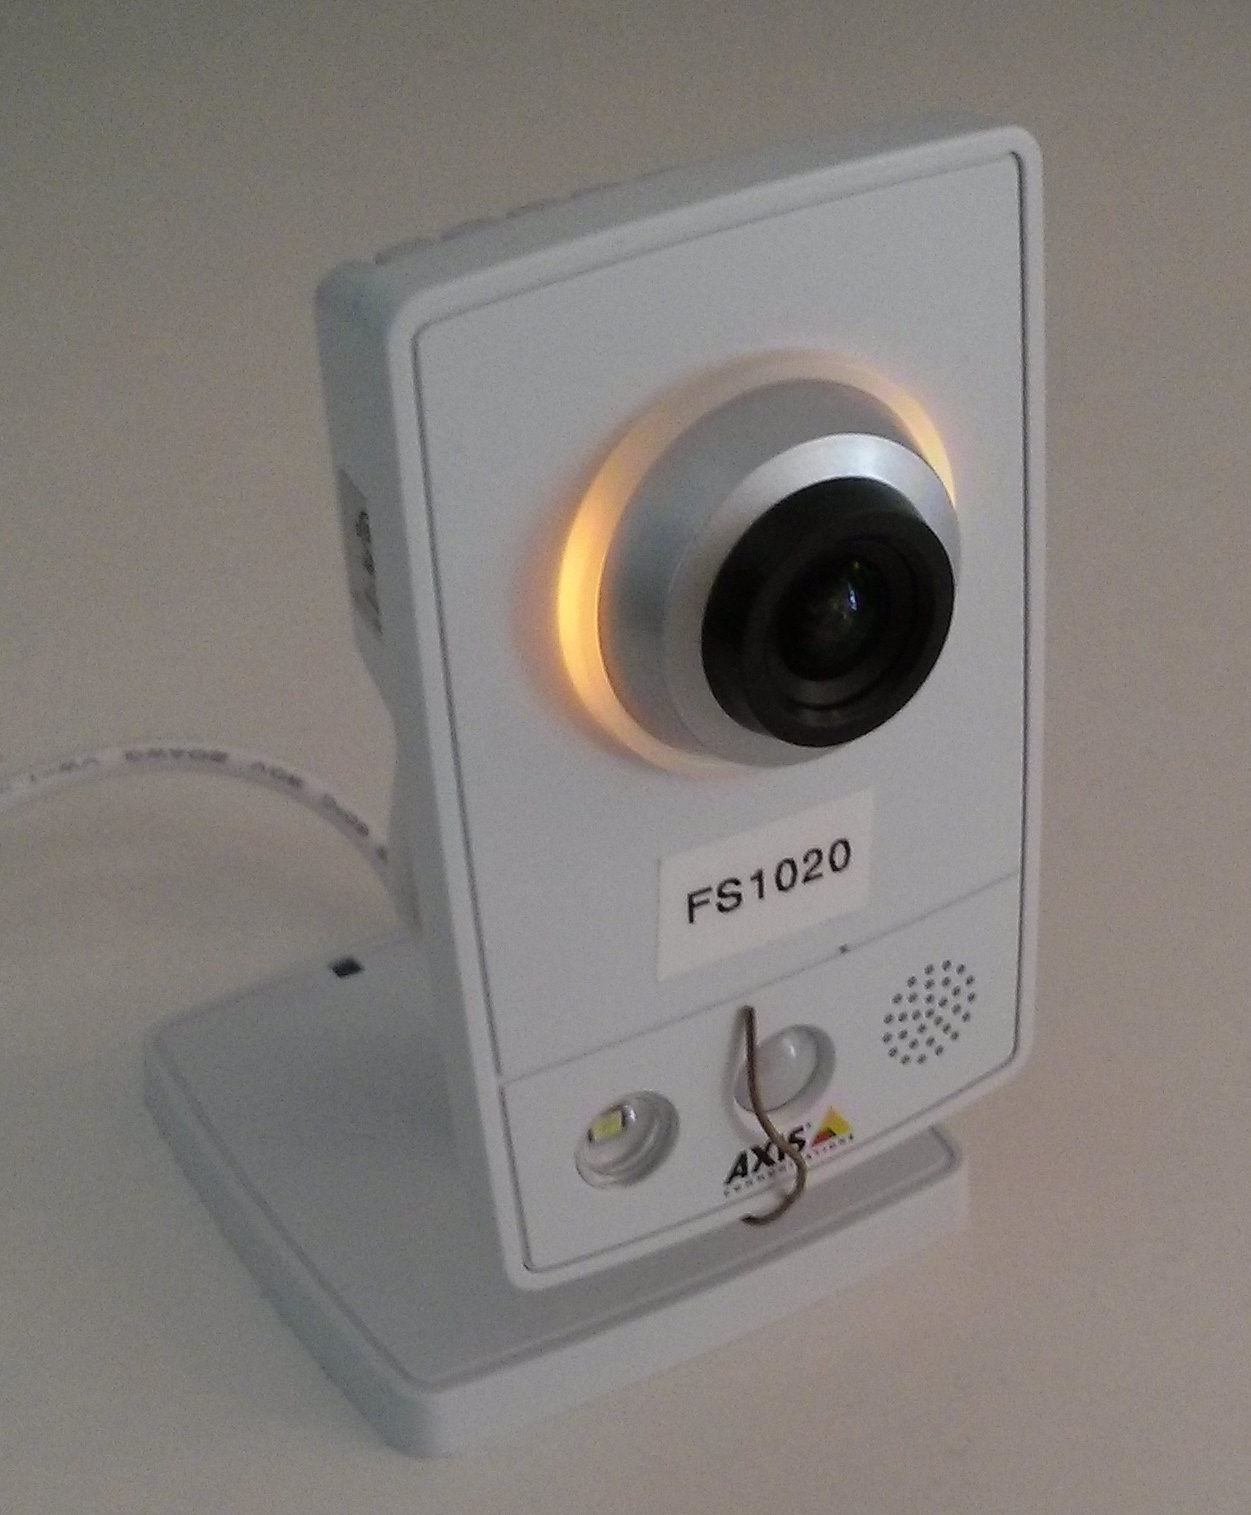
\includegraphics[width=0.5\textwidth]{m1033}
    \caption{The Axis M1033 camera}
    \label{fig:M1033}
\end{figure}

It is very likely, due to its capabilities, that multiple applications run
simultaneously on the hardware, especially due to the ability of recording 
and playing audio clips simultaneously. In fact, while the video is recorded
and sent over the network, it is also possible to run other applications
using the collected data, for example some motion detection application.

\subsection{Axis P3367}

The Axis P3367~\cite{p3367} is a fixed dome network camera capable of 
multiple H.264 streams as well as Motion JPEG streams. It supports 
various frame rates and resolutions up to 5 Megapixel at 12 frames per 
second, it also supports HDTV 1080p at 30 frames per second and has two 
way audio streaming capabilities.

\begin{figure}[h]
    \centering
    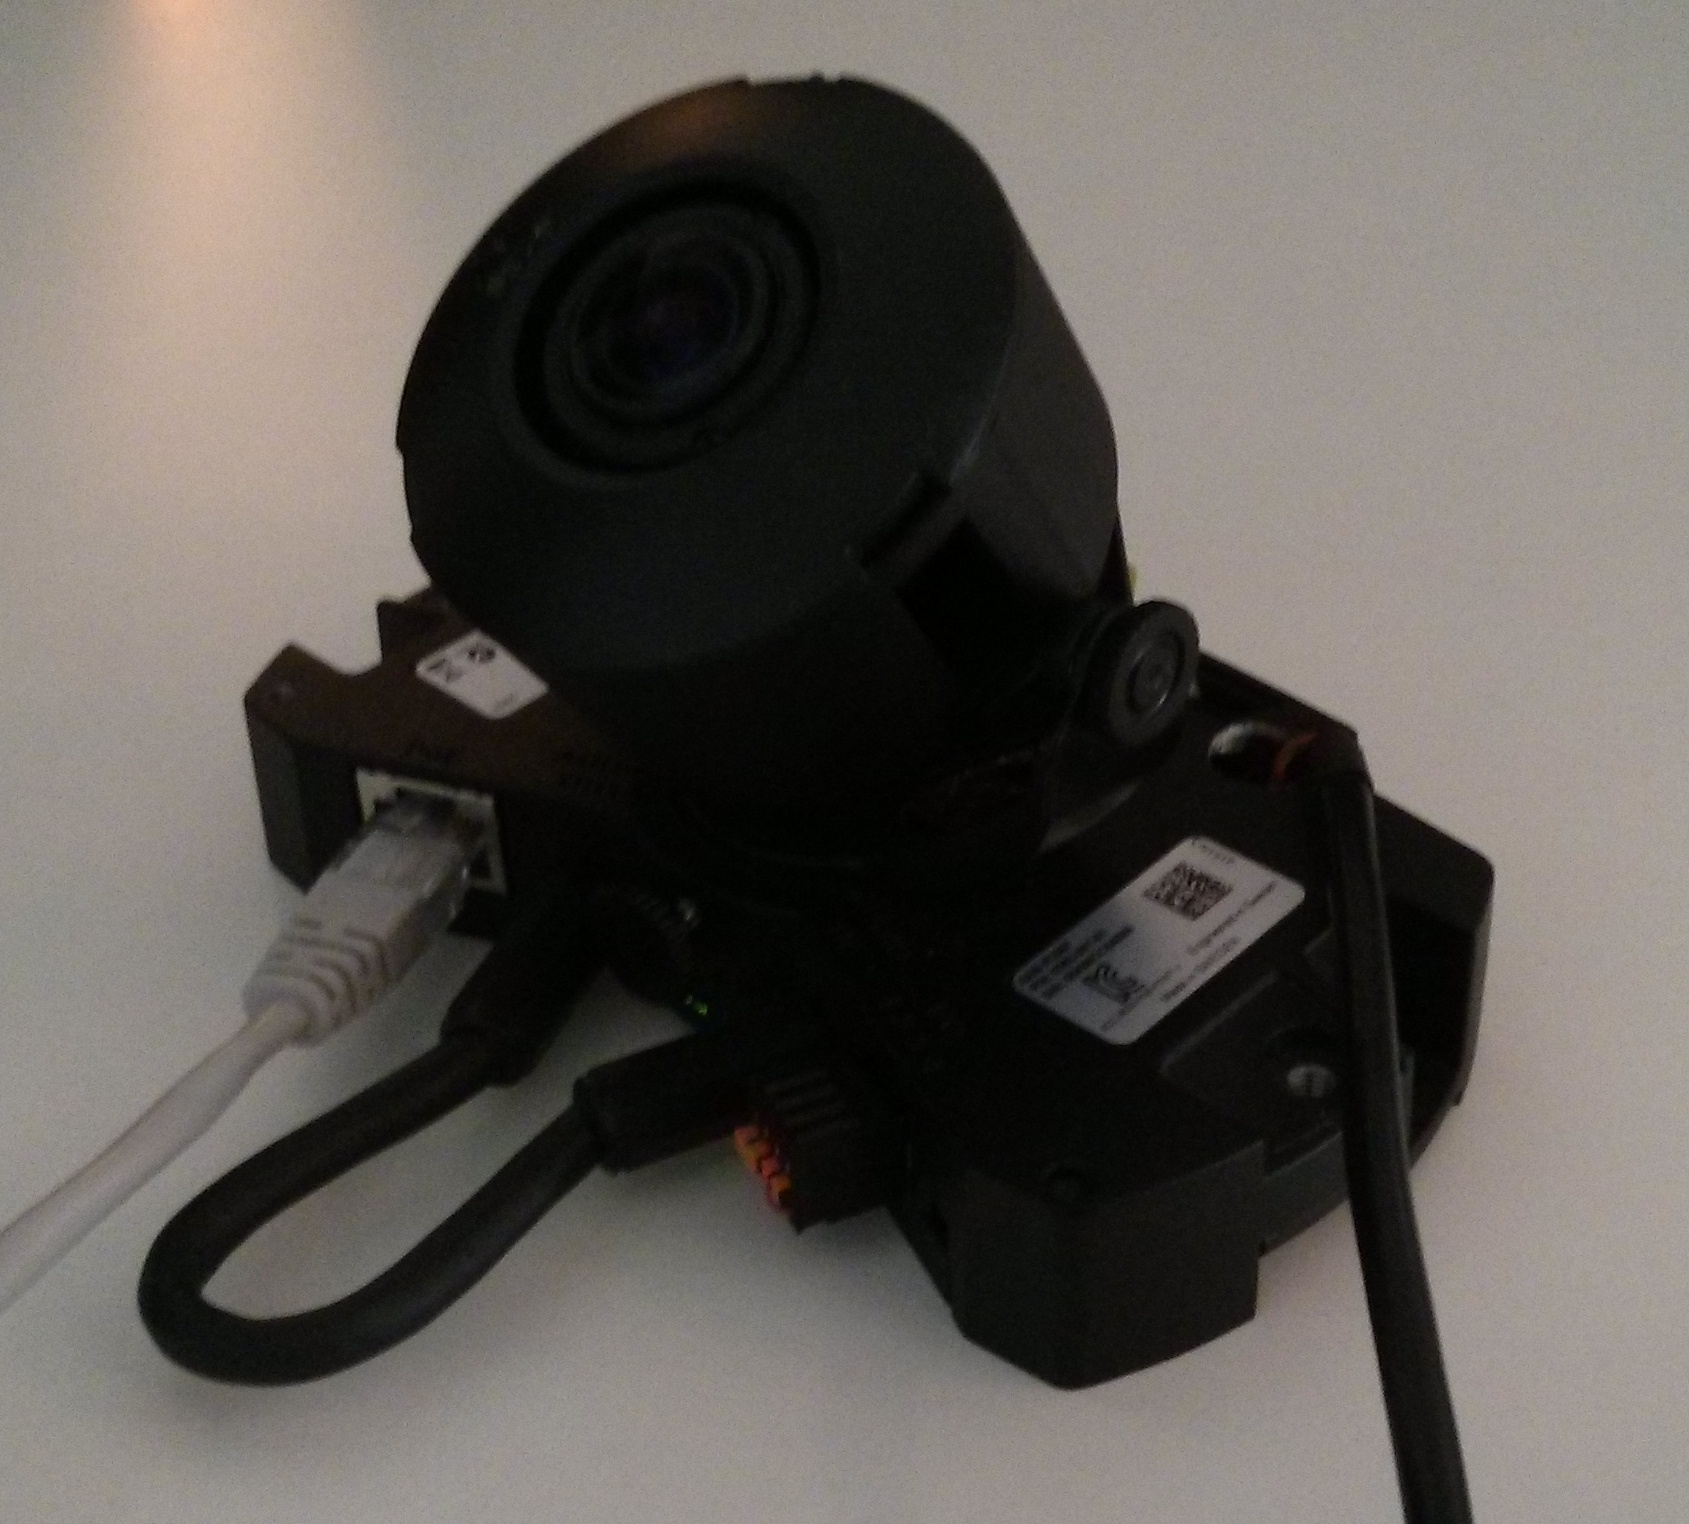
\includegraphics[width=0.5\textwidth]{p3367}
    \caption{The Axis P3367 camera, without its dome casing}
    \label{fig:P3367}
\end{figure}

\begin{figure}[h]
    \centering
    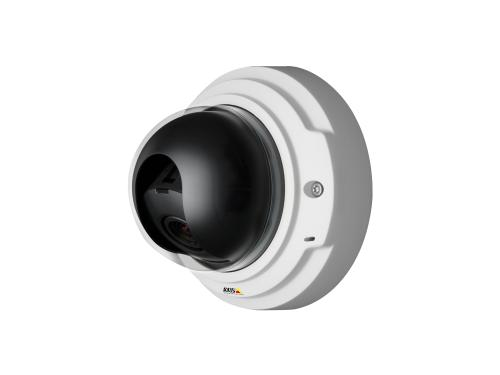
\includegraphics[width=0.5\textwidth]{p3367incase}
    \caption{The Axis P3367 camera, here in its final form}
    \label{fig:P3367}
\end{figure}

The power is supplied using Power over Ethernet, therefore the camera does 
not need a separate power supply and is powered directly through the network
cable. It features an ARTPEC-4~\cite{artpec-4} system-on-chip, developed 
by Axis, which contains a single-core CPU running at 400 MHz and a 
co-processor dedicated to video analytics.

It is clearly more advanced than the M1033 but it shares the same
characteristics of being extremely flexible to execute multiple applications
at the same time, especially due to the video analytics co-processor.

These cameras are very common amongst Axis' costumers and also by the 
developers and will serve as realistic testing platforms for this project. 
Initially the M1033 was the only camera considered but during development a 
later version of systemd was brought to the P3367 and the project moved to 
that camera instead. Testing will thus only be carried out only on the P3367 
as the previous cameras systemd implementation differs to much to bring the 
software to both of them.

\chapter{Implementation}
\label{chp:development}

This chapter describes the implementation of the GTRM framework for
Axis cameras. The code commented upon was written in C and cross-compiled 
using Axis' compiler for the corresponding hardware platform. The resource
allocation framework was testing in different use cases and with a
variety of service files and slices. The resulting plots are generated with
Octave.

\section{Design choices}

Introducing service levels in all the applications running on camera
is not a realistic approach. This is because there are many different
applications, some of which may not even be developed at Axis, and 
developers are not expected to modify all these applications to implement 
the performance measurements and service level features needed, despite the
modification being trivial in many cases. Also, for some applications it is
not possible to identify the concept of service level. 

The service level is in this work implemented for the video streaming
application and for some test application that generates mathematical load
in the system. This thesis only focuses on the implementation of GTRM and 
assumes that a correct implementation of the framework implies also that
the proof of convergence of the game theoretic strategy holds, as
demonstrated for~\cite{gtrm}.

Also, the service level assignment is limited to the linear case, where
resource requirements (in this case CPU requirements) are a linear function 
of the service level. It can be argued that the CPU requirement/SL
relationship can be linearized around a point and hence still considered
linear close to the operating point. 

The matching function used to determine the performance of the application is
time sensitive and reads as
\begin{equation}
f_{i}=\cfrac{D_{i}}{R_{i}}-1
\label{eq:matchingfunctiongeneral}
\end{equation}
where $D_{i}$ is the soft deadline for the job and $R_{i}$ is the job 
response time. This matching function is positive when the resource given is
aboundant and negative if it is scarce. It is also zero in case there
is a perfect match between the resource given and the service level set by
the application. The aim of GTRM is to bring $f_i$ to zero for all the
running applications. It is assumed that $f_i$ is measurable also for the
non-service level aware applications. The matching function is updated as
the average of the measured value for the last ten jobs.
\newstuff{Resource management in this paper is restricted to cpu, cgroups have a controller to handle memory management as well, the \emph{memory} controller, 
which is not installed on the camera.}

\section{Inter-Process Communication}

The resource manager is implemented within \texttt{systemd} and its code
is therefore integrated into the \texttt{systemd} code. If an application
has a poor matching function it should send information to \texttt{systemd}
via UNIX-sockets. The Inter-Process Communication (IPC) consists of one 
socket declared within the \texttt{systemd} code and one for each application
that the resource manager should monitor. 
The socket setup is inspired by the ``Notify'' feature of \texttt{systemd}
which is used by services that want to notify \texttt{systemd} that they 
have started or about status changes [sysd-notify].

\subsection{Retrieving new events}

The system uses \texttt{epoll} to find out which sockets has received new 
messages. The events returned from \texttt{epoll\_wait()} are then put in 
a prioritized queue. This first element in the prioritized queue is then 
dequeued, calling its callback function. This means that a message might 
not be read immediately after being retreived from the buffer. Most of the
functions used to manage \texttt{epoll} are located in \texttt{sd-event.c},
which serves as a wrapper for many different event, such as those generated by 
\texttt{epoll}.

The \texttt{epoll\_wait} prototype is
\begin{verbatim}
int epoll_wait(int epfd, struct epoll_event *events,
               int maxevents, int timeout);	 
\end{verbatim}
and the function behaves as follows. When there are messages to be read on 
one of the file descriptors observed by the \texttt{epoll} instance 
identified with the file descriptor \texttt{epfd}, the function returns 
the number of file descriptors that have new messages to be read. 

If this happens, \texttt{epoll\_event *events} points to a buffer that 
the function fills with the incoming events. The buffer in the end contains
a maximum of \emph{maxevents}. The function waits for a maximum
\texttt{timeout} value.

The \texttt{epoll\_event} structure follows.
\begin{lstlisting}
typedef union epoll_data {
  void    *ptr;
  int      fd;
  uint32_t u32;
  uint64_t u64;
} epoll_data_t;





<<<<<<< Updated upstream

=======
>>>>>>> Stashed changes
struct epoll_event {


  uint32_t     events; /* Epoll events */
  epoll_data_t data;   /* User data variable */
};
\end{lstlisting}

The void pointer \texttt{epoll\_event.data.ptr} will be set to point to a 
\texttt{sd\_event\_source} structure. This structure is the element that is
enqueued into the prioritized queue. The element contains information
concerning the event priority and defines the event type. It also point to
a structure containing the file descriptor for the event and its callback
function.

The function \texttt{sd\_event\_run} is called once for every iteration of
the main loop. The relevant code in this function is shown below.
\begin{lstlisting}
_public_ int sd_event_run(sd_event *e, 
  uint64_t timeout) {
  struct epoll_event *ev_queue;
  unsigned ev_queue_max;
  sd_event_source *p;
  int r, i, m,timeout;        
  ev_queue = new(struct epoll_event, ev_queue_max);
  m = epoll_wait(e->epoll_fd, ev_queue, 
    ev_queue_max,timeout);

  for (i = 0; i < m; i++) {
    if (ev_queue[i].data.ptr == 
        INT_TO_PTR(SOURCE_MONOTONIC))
      r = flush_timer(...);
    else if (ev_queue[i].data.ptr == 
        INT_TO_PTR(SOURCE_REALTIME))
      r = flush_timer(...)
    else if (ev_queue[i].data.ptr == 
        INT_TO_PTR(SOURCE_SIGNAL))
      r = process_signal(e, ev_queue[i].events);
    else if (ev_queue[i].data.ptr == 
        INT_TO_PTR(SOURCE_WATCHDOG))
      r = flush_timer(e, e->watchdog_fd, 
        ev_queue[i].events, NULL);
    else
      r = process_io(e, ev_queue[i].data.ptr, 
        ev_queue[i].events);
  }

  p = event_next_pending(e);
  r = source_dispatch(p);
  return r;
}
\end{lstlisting}

The \texttt{epoll\_wait} function is called and a for loop goes through 
all the file descriptors and checks what their event type is to call the
appropriate function to add them to the prioritized queue.
The GTRM file descriptor is linked to a \texttt{IO\_SOURCE} event which 
means that the function \texttt{process\_io()} will be called in case there
is an event on such file descriptor.

Subsequently, the next event is dequeued from the queue and dispatched by
calling \texttt{event\_next\_pending()}. The code of this function is
shown below.
\begin{lstlisting}
static sd_event_source* 
  event_next_pending(sd_event *e) {
	  sd_event_source *p;
  	p = prioq_peek(e->pending);
  	if (!p)
  		  return NULL;
  	if (p->enabled == SD_EVENT_OFF)
  		  return NULL;
  	return p;
}
\end{lstlisting}
Finally, the \texttt{source\_dispatch} function is called to activate 
the callback function linked to the top \texttt{sd\_event\_source*} 
element.
\begin{lstlisting}
static int source_dispatch(sd_event_source *s) {
	int r = 0;
	switch (s->type) {
  	case SOURCE_IO:
  		  r = s->io.callback(s, s->io.fd, 
          s->io.revents, s->userdata);
  		  break;
  	case SOURCE_MONOTONIC:
  		  r = s->time.callback(s, s->time.next, 
          s->userdata);
  		  break;
  	case SOURCE_REALTIME:
  		  r = s->time.callback(s, s->time.next, 
          s->userdata);
  		  break;
  	/* More cases covered */
  	case SOURCE_WATCHDOG:
  		  assert_not_reached("Wut? I shouldn't exist.");
	}
	return 1;
}
\end{lstlisting}

\subsection{The GTRM socket}

The socket used by the applications to communicate with the resource
manager and by the resource manager to retrieve information about the
application health is setup as follows.

The socket is created and added to the \texttt{epoll} instance in the
function \texttt{manager\_setup\_gtrm}, some information about it
follows.

\begin{framed}
	\begin{flushleft}
		\textbf{\emph{{static int manager\_setup\_gtrm(Manager *m)}}} 
    \newline
		Used to setup the socket, event source and file descriptor for the
    resource manager. Called from \texttt{manager\_startup} and 
    \texttt{manager\_reload}.
		\begin{itemize}
		\item m: Reference to the manager.
		\item Return value: Zero if function ran correctly, otherwise it is 
      set to the corresponding error number.
		\end{itemize}
	\end{flushleft}	
\end{framed}

This function contains the socket creation, obtained through
\texttt{socket}:
\begin{verbatim}
fd = socket(AF_UNIX, 
  SOCK_DGRAM|SOCK_CLOEXEC|SOCK_NONBLOCK, 0);
\end{verbatim}
The socket uses the protocol family \texttt{AF\_UNIX}, which provides
efficient communication on the same machine. \texttt{SOCK\_DGRAM} sets 
the socket type to be datagram since there is no need to resend missed
obsolete data and no messages are expected to be lost when sent over the 
same machine. \texttt{SOCK\_NONBLOCK} prevents the socket from blocking 
during a \texttt{read} call when there is no data to be read. A random 
address name is created and assigned to the socket by a call to 
\texttt{bind}. The file descriptor of the socket is then added to the 
\texttt{epoll} instance, and an \texttt{epoll\_event} is associated to
the file descriptor. The \texttt{epoll\_event} contains a pointer to 
an \texttt{sd\_event\_source}. These functionalities are achieved through
the call to \texttt{sd\_event\_add\_io}.

\begin{verbatim}
r = sd_event_add_io(m->event, &m->gtrm_event_source, 
  m->gtrm_fd, EPOLLIN, manager_dispatch_gtrm_fd, m);
\end{verbatim}

The GTRM socket has been therefore added to the poll and a corresponding 
event is subsequently generated whenever a message is sent to that socket. 
Finally, in the function \texttt{manager\_setup\_gtrm} a priority is given
to the \texttt{gtrm\_event\_source}. This affects how the prioritized 
queue sorts messages from this source type and the priority is set equally
to the priority for notify messages.

Once the socket is setup and ready, a environment variable is set in 
Linux containing the address to the GTRM-socket. The environment variable is
used by the applications to retrieve the destination of the messages to be
sent about their performance.

\subsubsection{GTRM socket's callback function:}
Once an event has been popped from the prioritized queue the callback 
function \texttt{manager\_dispatch\_gtrm\_fd} is invoked. 
The callback function contains all the code that should be executed when a
message is received on the GTRM socket. The function extracts the data 
from the message --- the PID of application sending the message, its
performance and its weight. The \texttt{hashmap}, which contains all the
applications that are managed by GTRM, is then updated with this new data. 

\begin{framed}
	\begin{flushleft}
		\textbf{\emph{static int manager\_dispatch\_gtrm\_fd \newline
      (sd\_event\_source *source, int fd, unit32\_t revents, void *userdata)}} \newline 
			Called upon receiving the performance of an application.
			\begin{itemize}
			\item source: source of the event.
			\item fd: file descriptor to the event source.
			\item revents: Set by the kernel to indicate what event on the file
        descriptor that triggered the call to this function. For the purposes
        of this work, it is always the incoming event.
			\item userdata: Contains a reference to the manager.
			\item Return value: Not used, always zero.
			\end{itemize}
	\end{flushleft}	
\end{framed}

The function contains some declaration and initialization.
\begin{lstlisting}
static int manager_dispatch_gtrm_fd
  (sd_event_source *source, int fd,
  uint32_t revents, void *userdata) {
  Manager *m = userdata;    		    
  char buf[1024]; // read message
  int n; // byte size of the read message
  struct sockaddr_un *from; // sender's adress
  socklen_t fromlen;
  rm_app_t *app; // data about the applications
  rm_app_t *app2;	
  fromlen = 1024;
  ... // will be shown later
\end{lstlisting}

Within the function, the \texttt{rm\_app\_t} structure is used.
\begin{framed}
	\begin{flushleft}
		\textbf{\emph{struct rm\_app\_t}}
		Represents an application being managed and consists of the 
    following fields.
		\begin{itemize}
		\item tid: Applications PID.
		\item vp: Virtual platform.
		\item vp\_old: Previous virtual platform.
		\item performance: Matching function of the application.
		\item weight: The current ``weight'' of the application.
		\item happy: Indicates if the application is happy with its 
      current performance. This field was added to prevent application from
      sending their performance even when they are satisfied and nothing 
      should be needed from the resource manager, eliminating unnecessary 
      computations.
		\item sa: Socket Address, used to send back the performance 
      multiplier.
		\end{itemize}
	\end{flushleft}	
\end{framed}

A while loop reads the socket one message at a time, until there are no 
more unread messages. 

\begin{lstlisting}
  // resuming from above
  do {		
  	memset(buf, '\0', 1023);
  	from = calloc(1, sizeof(struct sockaddr_un));
  	app = calloc(1, sizeof(rm_app_t));	
  	n = recvfrom(fd, buf, 1024, 0, 
      (struct sockaddr *) from, &fromlen);
    // with non-blocking sockets
  	// if n is negative, there was no message
  	n = recvfrom(fd, buf, 1024, 0, 
      (struct sockaddr *) from, &fromlen);
  	if (n<0)
  		break;
  	if (n>1024) // reading 1024 characters at a time
  		log_error("manager_dispatch_gtrm_fd:
        received too big message");

  	gtrm_char2gtrmstruct(buf, app);
  	pid_t pid = app->tid;
  	app->sa = from;
  	if(hashmap_get(m->gtrm_apps, pid) == NULL) {
  		hashmap_put(m->gtrm_apps, pid, app);
  	} else {
  		app2 = hashmap_get(m->gtrm_apps, pid);
  		gtrm_update_rm_struct(app,app2);
  	}															
  } while(n>0);
  m->update_gtrm = true;
  return 0;
}
\end{lstlisting}

The data contained in the message is used to create a \texttt{rm\_app\_t}
structure. If the hashmap already contains a \texttt{rm\_app\_t} structure 
for the specific application, the \texttt{rm\_app\_t} in the hashmap is
simply updated by calling the function 
\texttt{gtrm\_update\_rm\_struct(app,app2)}. In the opposite case, the new
application is added to the hashmap using the application PID as the key.

Above, a few library function contained in \texttt{gtrm\_lib} were used.
In particular, the \texttt{gtrm\_char2gtrmstruct} function is used to
convert the information between the received string and the GTRM
compliant structure.
\begin{framed}
	\begin{flushleft}
		\textbf{\emph{void gtrm\_char2gtrmstruct(char* str, rm\_app\_t *re)}}
		Extracts data from a received string and store it as a structure 
    instead. The data sent from an application consists of the PID,
    performance, weight and if the application is satisfied or not.
		\begin{itemize} 
		\item str: String to extract data from.
		\item re: Struct to hold the extracted data.
		\item Return value: None, the result is stored in re.
		\end{itemize}
	\end{flushleft}	
\end{framed}

\subsection{Resource Manager Update}
The resource manager is recomputing the amount of resource to be given to
the applications, and reapplied until the applications are not completely
satisfied. The following code is contained inside the 
\texttt{manager\_loop}-function of \texttt{manager.c}.

\begin{lstlisting}
int manager_loop(Manager *m) {
\end{lstlisting}

Before the loop actually starts to run, a structure that contains the
necessary data for the resource manager, \texttt{gtrm\_t}, is created 
and initialized.

\begin{framed}
	\begin{flushleft}
			\textbf{\emph{{struct gtrm\_t}}} \newline
			Stores various parameters used by the GTRM.
			\begin{itemize}
			\item c1: Constant used for computing $\epsilon$, determines how much 
        the virtual platforms will be changed.
			\item c2: Another constant used for computing epsilon similar as c1.
			\item iterations: Keeps track of how many iterations the GTRM has run.
			\item all\_happy: Used to indicate if we have to make any adjustments 
        to the resource allocations.
			\item num\_apps: Total amount of applications that we are managing.
			\item prev\_apps: The amount of applications in the previous iteration.
			\end{itemize}
	\end{flushleft}	
\end{framed}

\begin{lstlisting}
  gtrm_t *gtrm_t = calloc(1,sizeof(struct gtrm_t));
  gtrm_t->num_apps = 0;
  gtrm_t->prev_apps = 0;
  gtrm_t->iterations = 0;
  gtrm_t->all_happy = true;
  gtrm_t->c1 = 0.1;
  gtrm_t->c2 = 10;
  while (m->exit_code == MANAGER_RUNNING) {
  ...
\end{lstlisting}
Inside the loop, an if-statement makes sure that the resource manager is not run if not needed. 
\begin{lstlisting}
    if ((!(gtrm_t->all_happy) || m->update_gtrm) && 
      !hashmap_isempty(m->gtrm_apps)) {
\end{lstlisting}

The first step is to update the number of running applications.
\begin{lstlisting}
      gtrm_t->prev_apps = gtrm_t->num_apps;
      gtrm_t->num_apps = hashmap_size(m->gtrm_apps);
\end{lstlisting}

\begin{framed}
	\begin{flushleft}
			\textbf{\emph{{int gtrm\_compute\_virtual\_platforms \newline
      (Hashmap *apps, gtrm\_t *gtrm\_t)}}} \newline
			Calculates the amount of resources (virtual platform) for an application.
			\begin{itemize}
			\item apps: The hash-map containing information about the
        applications being managed.
			\item gtrm\_t: Struct with parameters used when calculating the 
        virtual platforms.
			\item Return value: Not used, always zero.
			\end{itemize}
		\end{flushleft}	
\end{framed}

\begin{lstlisting}
      gtrm_compute_virtual_platforms
        (m->gtrm_apps, gtrm_t);
      gtrm_t->iterations++;
\end{lstlisting}

The virtual platforms are then applied to the applications and a variable set by the dispatch is reset to false.
\begin{framed}
	\begin{flushleft}
			\textbf{\emph{{void gtrm\_apply\_virtual\_platforms(Manager* m)}}}
      \newline
			Computes and applies the amount of CPUShares that each application 
        shall be given.
			\begin{itemize}
			\item m: Reference to manager, used to get the applications
			\item Return value: None.
			\end{itemize}
	\end{flushleft}	
\end{framed}
\begin{lstlisting}
      gtrm_apply_virtual_platforms(m); 
      m->update_gtrm=false;																	
\end{lstlisting}

The final step inside the loop is to update the performance multiplier to be
provided to the applications and log the relevant data.
\begin{framed}
	\begin{flushleft}
			\textbf{\emph{{void gtrm\_update\_performance\_multipliers \newline
      (int gtrm\_fd, Hashmap *gtrm\_apps)}}} \newline
			Calculates, updates and sends the performance multiplier to 
      each application, using the performance, virtual platform and 
      the previous virtual platform for each application.
			\begin{itemize} 
			\item gtrm\_fd: File descriptor used to send the performance 
        multiplier.
			\item gtrm\_apps: Hash-map containing rm\_app\_t structs for 
        each application.
			\item Return value: None.
			\end{itemize}
	\end{flushleft}	
\end{framed}

\begin{framed}
	\begin{flushleft}
		\textbf{\emph{{void gtrm\_write\_log \newline
    (Hashmap *gtrm\_apps, unsigned int num\_applications)}}} \newline
		Writes information about the resource management to a log file, 
    which can then be used to generate graphs about the applications
    behavior and the resource manager allocation.
		\begin{itemize} 
		\item gtrm\_apps: Hash-map containing rm\_app\_t structs for 
      each application.
		\item num\_applications: Used to make sure we don't try to print 
      an empty hash-map.
		\item Return value: None.
	  \end{itemize}
  \end{flushleft}	
\end{framed}

\begin{lstlisting}
      gtrm_update_performance_multipliers
        (m->gtrm_fd,m->gtrm_apps);
      gtrm_write_log(m->gtrm_apps, gtrm_t->num_apps);
    }
  }
\end{lstlisting}

If the loop exits it is necessary to deallocate the \texttt{gtrm\_t} 
structure to avoid memory leaks.
\begin{lstlisting}
  free(gtrm_t);
  return m->exit_code;
}
\end{lstlisting}

\subsection{Applying the virtual platforms}

The computed values for the virtual platforms need to be distributed to 
the applications. This is achieved via the following function.
\begin{lstlisting}
void gtrm_apply_virtual_platforms(Manager* m) {
\end{lstlisting}

Three variables are defined for setting the shares, iterating through 
the hashmap and a structure for each application.
\begin{lstlisting}
  int shares;
  Iterator i;
  rm_app_t* a;
\end{lstlisting}

\texttt{HASHMAP\_FOREACH} is a macro defined in \texttt{hashmap.h} and it is
used to easily iterate through all the elements in the hashmap. 
The macro takes three parameters, a local variable to store the current
element in the iteration, the hashmap to iterate through and an iterator.
\begin{lstlisting}
  HASHMAP_FOREACH(a, m->gtrm_apps, i) {
\end{lstlisting}
Since the virtual platform is given as a percentage of the total amount of
available resource, each application's virtual platform is multiplied by a
constant, \texttt{\_TOTAL\_SHARES}, to give the absolute amount of shares.
\begin{lstlisting}
    shares = a->vp * _TOTAL_SHARES;
    manager_set_cpu_shares(m, a->tid, shares);
  }
}
\end{lstlisting}
Finally the CPUShares of the application is set, end then the loop repeats
until all the applications in the system have been updated.

\begin{framed}
	\begin{flushleft}	
		\textbf{\emph{{int manager\_set\_cpu\_shares(Manager *m, pid\_t pid, int shares)}}} \newline
		Sets the CPUShares of an application.
		\begin{itemize}
		\item m: Reference to manager, used to get the applications.
		\item pid: Process identifier of the application.
		\item shares: Amount of shares we want to set.
		\item Return value: Zero if successful, one otherwise.
		\end{itemize}
	\end{flushleft}	
\end{framed}

\subsection{Setting CPUShares}
From the command line one can manually set the amount of CPUShare of 
an application by running the command, 
\texttt{systemctl set-property 'service name' CPUShares='shares'} followed 
by \texttt{systemctl daemon-reload}. These commands take a lot of time since
they involve calls via \texttt{DBus} to \texttt{systemd}. That is the reason
why in this work the resource manager itself is located within 
\texttt{systemd}, so that these calls can be circumvented, by setting 
the CPUShares directly.

\begin{lstlisting}
int manager_set_cpu_shares(Manager *m, pid_t pid, int shares){
\end{lstlisting}
Two local variables are needed, a pointer to a \texttt{Unit} and one to a 
\texttt{CGroupContext}. From the PID of an application, the corresponding 
Unit pointer can be obtained.
\begin{lstlisting}
  Unit* u;
  CGroupContext* c;
  u = manager_get_unit_by_pid(m, pid);
\end{lstlisting}
In case the application does not exist, because the application terminated,
the Unit pointer produced previously will be a NULL-pointer. The application
is thus removed from the hashmap, which requires that we reset the virtual
platforms, and the function call returns.
\begin{lstlisting}
  if(u == NULL) {
    hashmap_remove(m->gtrm_apps, pid);
    reset_virtual_platforms(m->gtrm_apps);
    return 1;
  }
\end{lstlisting}

If the Unit-pointer obtained was not NULL, a so called \texttt{CGroupContext}
can be acquired from the Unit-pointer.
\begin{lstlisting}
  c = unit_get_cgroup_context(u);
\end{lstlisting}
In this context, the CPUShares can be set to what is desired and it is
followed be a necessary call to apply the changes.
\begin{lstlisting}
  c->cpu_shares = shares;
  cgroup_context_apply(c, CGROUP_CPU, u->cgroup_path);
  return 0;
}
\end{lstlisting}

In Section~\ref{sec:systemdandcroups} we introduced CPUShares, which assigns 
CPU-resources between the application proportionally to the amount of shares 
assigned to each application. This implies that assigning an application an 
amount of shares, will give different amount of resources depending on how the 
shares are assigned to the competing applications. The CPUShares also define a 
minimum amount of resources, an application can thus receive more resources 
than specified if there is free resources available. This is different to the 
approach in~\cite{gtrm} where the resources where set exact via 
\texttt{SCHED\_DEADLINE}. Some risks are introduced by using 
\texttt{SCHED\_DEADLINE} which are not present in the CPUShares approach. Such 
as assigning, in total, more resources than available, causing a kernel-panic 
or not fully utilizing the system by assigning less resources, in total. 
\texttt{SCHED\_DEADLINE} also has to take the amount of CPU cores into 
consideration, which CPUShares is independent of.


\section{Service Level Update}
\label{sec:servicelevelupdatesection}

The applications using the GTRM framework have all a similar structure,
the main difference being how they implement the update in the service
level to match the resource allocation. In fact, the service level changes
are mapped into some parameter changes, that in turn affect the resource
requirement. This is different on a per application basis and every
application developer knows better what to change within the application
to make it require less or more resource and provide a worse or better
quality of service.

In general, however, a few elements can be identified. The service level
adaptation should run periodically and a socket nees to be established
and read during the adaptation phase. Below, we show an example of
test application, to show how the service level adaptation can be performed
and what functions are provided by \texttt{gtrm\_app\_lib.c}.
The test application and library are altered versions of the test 
application and library \texttt{jobsignaler.c} used within~\cite{gtrm}.
The modifications are mainly due to the presence of sockets, instead of
the initial shared memory approach used by \texttt{jobsignaler}.

\begin{lstlisting}
// Initial declarations, some not reported
// because irrelevant [...]
uint id;
_application_h* myself;
...	

int main (int argc, char* argv[]) {
	// parsing information from char* argv[].
	float service_level;
	float a_cpu, b_cpu;
	float a_mem, b_mem;
	double epsilon, weight;
	double deadline_seconds;
	
	int jobs;
	double performance;
\end{lstlisting}

The application creates the socket adress and pass it as an argument to 
\texttt{gtrm\_lib\_setup\_socket}. The file descriptor is then linked to
a file with the application name.
\begin{lstlisting}
	char* sock_path = "/root/temp/app";
	unsigned int r_nbr = random_u64();
	char* sock_name[100];
	sprintf(sock_name,"%s/%u",sock_path,r_nbr);
	gtrm_lib_setup_socket(sock_name);
\end{lstlisting}

\begin{framed}
	\begin{flushleft}		
		\emph{\textbf{{int gtrm\_lib\_setup\_socket(char* filename)}}}
		Sets up a socket to communicate with the resource manager. 
    Reads an environment variable set by \texttt{systemd} for the GTRM
    socket adress and creates a socket adress struct.
		\begin{itemize}
		\item filename: The socket needs a file to work, the parameter 
      specifies its path.
		\item Return value: Zero, not used.
		\end{itemize}
	\end{flushleft}
\end{framed}

Subsequently the arguments for the \texttt{gtrm\_lib\_set} function
are initialized and passed.
\begin{lstlisting}	

	myself->weight = weight;
	myself->application_id = getpid();
	uint64_t deadline = (unsigned int) 
    ((double)1000000000 * deadline_seconds);
	uint64_t ert[1] = {deadline};
	gtrm_lib_set(myself, 1, ert);
\end{lstlisting}
Applications can have different job types corresponding to different 
deadlines within the same code. For example, this is the case of a video
decoder/encoder, that could process different types of frames (I/B/P)
with different requirements. Encoding an I frame requires to simply
transfer the information from one place to the other, while encoding a B and
P frame, in fact, require to compute the differences between the previous
I frame and eventually the subsequent ones. The test application has 
only one job type but the framework directly supports multiple job types. 
An application can have different job types corresponding to different deadlines. The test application only has one job type. 

\begin{framed}
	\begin{flushleft}		
		\emph{\textbf{{int gtrm\_lib\_set
    (\_application\_h* a, uint types, uint64\_t* ert)}}} \newline
		Initializes the application struct with job types and their 
    expected response times.
		Initializes the application struct with job types and their expected response times.
		\begin{itemize}
		  \item a: Struct representing an application.
		  \item types: Number of different job types.
		  \item ert: Array of expected response time for each job type.
		  \item Return value: Exit status of function.
    \end{itemize}
  \end{flushleft}
\end{framed}

The main loop of the program follows.

\begin{lstlisting}
	for(;;) {		
		int64_t cpu_requirement = a_cpu * service_level 
      + b_cpu;
		int64_t mem_requirement = a_mem * service_level 
      + b_mem;
		int type = 0;
		id = gtrm_lib_jobsignaler_signalstart
      (myself, type);		
		// Do the required work	
		do_work(cpu_requirement, mem_requirement, 
      NOISE_PERCENTAGE);	
		gtrm_lib_jobsignaler_signalend(myself, id);
		id = 0;										
		performance = gtrm_lib_get_performance_number
      (myself, type);
		
		// Adapt only if needed
		if (performance < -0.01 || performance > 0.01) {
			myself->happy = false;					
			// send performance to systemd
			gtrm_lib_send_performance(myself, performance);					
			// if there is no multiplier to read use the 
      // simple service level adaption
			if (gtrm_lib_update_performance_multiplier
          (myself) == 0)
				service_level += epsilon * service_level *
          (myself->performance_multiplier-1);
			else
				service_level += epsilon * 
          (performance * service_level);	
		  // saturation											
			if (service_level < MINIMUM_SERVICE_LEVEL)
				service_level = MINIMUM_SERVICE_LEVEL;
			if (service_level != service_level) // avoid nans
				service_level = 1.0;
		} else if(myself->happy == false) {			
			myself->happy = true;
			gtrm_lib_send_performance(myself, performance);
		}	
	}	
}
\end{lstlisting}

In the code, the following functions are used.
\begin{framed}
	\begin{flushleft}		
		\emph{\textbf{{int gtrm\_lib\_signalstart
      (\_application\_h* a, uint type)}}} \newline
				Indicates the start of a job.
				\begin{itemize}
				\item a: Struct for representing the application.
				\item type: Type of the job that is started.
				\item Return value: Identifier of the started job.
				\end{itemize}
	\end{flushleft}
\end{framed}


\begin{framed}
	\begin{flushleft}	
			\emph{\textbf{{int gtrm\_lib\_signalend
        (\_application\_h* a, uint id)}}} \newline
			Indicates the end of a job.
			\begin{itemize}
			\item a: Struct for representing the application.
			\item id: Identifier of the job that has completed.
			\item Return value: Exit status.
			\end{itemize}
	\end{flushleft}
\end{framed}

\begin{framed}
	\begin{flushleft}	
		\emph{\textbf{{double gtrm\_lib\_get\_performance\_number \newline
    (\_application\_h* a, int job\_type)}}} \newline
		Calculates the peformance (matching function) by averaging 
    the performance of the last ten jobs of a specified type.
		\begin{itemize}
		\item a: Struct representing an application.
		\item type: Which job type for which we want to calculate 
      the performance.
		\item Return value: Applications performance.
		\end{itemize}
	\end{flushleft}
\end{framed}

\begin{framed}
	\begin{flushleft}	
		\emph{\textbf{{int gtrm\_send\_performance\_multiplier \newline
    (double pm, int fd, struct sockaddr *sa)}}} \newline
		Sends a performance multiplier to an application via sockets.
		\begin{itemize} 
		\item pm: Performance multiplier to send.
		\item fd: File descriptor used to send the performance multiplier.
		\item sa: Socket address.
		\item Return value: Always zero.
		\end{itemize}
	\end{flushleft}
\end{framed}

\section{Video Streaming}

This work features the modification of the video streaming application,
that is still undergoing. The proposed solution and implementation is
discussed here.

The streaming service, named \texttt{Monolith}, streams both video and 
audio. It handles image compression and filtering, manages several different
streams, such as H.264 and MJPEG streams. This application has been modified
to implement the service-level feature. The service level alters the image
quality by modifying the pipeline to prepare the frame for the video
streaming service.

In this pipeline an ``identity'' element is added. The identity element
forwards the received frames to the next element without affecting them.
This element is added just after the first (source) element.
The identity element calls a callback function by sending a ``handoff'' 
signal each time it receives a new buffer, where a buffer can contain one or 
more frames.

The time in between each incoming buffer to the identity element is the 
``job time'' for the streaming application, which is used when calculating the 
matching function, see Equation~\eqref{eq:matchingfunctiongeneral}. 
If a buffer contains only one frame, this job time should correspond to 
\emph{fps} on the camera.

After the matching function is computed, it is possible to calculate a new
service level for the application and to notify the resource manager. The
computed service level is then used to set the desired bit-rate in the 
bit-rate controller.

The bit-rate represents the amount of data that flows through the
application, measured in kbit per second. A higher bit-rate results in an
improved image quality, since more data is transmitted per frame. This is
obtained at the cost of higher computation time. When resources are limited,
the bit rate can be reduced allowing to restore a higher frame rate.

The bit-rate controller tries to match a specific bit-rate, despite how
the frame looks like. When the scenery becomes more complex, the bit-rate
will suddenly rise. There are two ways to cope with this: either the image
quality is reduced (by acting on the compression rate of the frame) or 
the frame rate is lowered. When one of these two actions is applied, the 
bit-rate will adjust to the desired level. The choice of the strategy to 
use is decided by setting the bit-rate priority field in \texttt{video.c}.

\begin{framed}
	\begin{flushleft}	
		\emph{\textbf{{void setup\_sl\_adapt \newline
    (float service\_level, double epsilon, double weight, double deadline\_seconds)}}} \newline
		Sets up deadline for computing the matching function and sets up the 
    Inter-Process Communication with the resource management.
		\begin{itemize}
		\item service\_level: Initial service level.
		\item epsilon: Constant which specifies service level adaptation rate.
		\item weight: Determines how the much of the adaptation will be done 
      by altering the service level or the changing the amount of resources.
		\item deadline\_seconds: This deadline will correspond to the 

      desired frame rate.
		\item Return value: None.
	\end{itemize}
	\end{flushleft}
\end{framed}

\begin{framed}
	\begin{flushleft}	
		\emph{\textbf{{void sl\_adapt()}}}
		Performs the service level adaptation, notifies the resource manager 
    and writes some logging.
		\begin{itemize}
		\item Return value: None.
		\end{itemize}
		\end{flushleft}
\end{framed}

The function which initiates the video pipeline is called 
\texttt{cache\_video} and is located in \texttt{video.c}. The function code
is quite complex but here we describe only what the features that are
relevant for this thesis.

\begin{lstlisting}
static GstElement *
cache_video (gpointer key, Props * props, 
  gpointer * user_data) {
  // Initialization and variable definitions
\end{lstlisting}

First, all the different elements belonging to the pipeline are defined,
including the newly introduced identity element, which is called 
\texttt{gtrm\_sl\_adapt}. A call to \texttt{setup\_sl\_adapt} sets
the variables needed for the service level adaptation.

At first all the different elements for the pipeline is defined, including the identity element, which is called \emph{gtrm\_sl\_adapt}. A call to \emph{setup\_sl\_adapt} sets up the what is needed for the service level adaptation.
\begin{lstlisting}
  GstElement *gtrm_sl_adapt = NULL;
  setup_sl_adapt (service_level, epsilon, 
    weight, deadline_seconds);
\end{lstlisting}

The identity element is created by the following calls and the 
\texttt{hand-off-signal} of the element is enabled and set up.

\begin{lstlisting}
  gtrm_sl_adapt = gst_element_factory_make 
    ("identity", "gtrm");
  g_object_set (G_OBJECT (gtrm_sl_adapt), 
    "signal-handoffs", TRUE, NULL);
  g_signal_connect (gtrm_sl_adapt, "handoff", 
    G_CALLBACK (gtrm_sl_cb), src);
\end{lstlisting}

Finally, the element must be inserted into the pipeline. This is obtained
via the following calls.

\begin{lstlisting}
  gst_bin_add_many(GST_BIN (p), src, gtrm_sl_adapt, 
    convert, caps_filter, sink, NULL);
  // More parameter definition here
  gst_element_link_many (src, gtrm_sl_adapt, convert, 
    caps_filter, sink, NULL);
}
\end{lstlisting}

The callback function for the element consists of a single call 
to \texttt{sl\_adapt()}, which is defined in \texttt{sl\_adapt.c}. 
This adaptation looks more or less identical to that in the test 
application described in Section~\ref{sec:servicelevelupdatesection} and
in Equations~\eqref{eq:servicelevelsimple} 
and~\eqref{eq:servicelevelnotsimple}.

\begin{lstlisting}
static void gtrm_sl_cb (GstElement * identity, 
  GstBuffer * buf, GstElement * src) {
  sl_adapt();
}
\end{lstlisting}

\section{Resource Allocation}

The resource allocation mechanism is realized using \texttt{cgroups},
\texttt{CPUShares} and \emph{slices}. Using slices one can set a minimum
amount of available resources for the applications that belong to the slice.

If the applications under a slice do not use all of the resources allocated 
to them, the unused share is free to be used by other slices. In a
hierarchical manner, each slice can have sub-slices, therefore dividing the resource at a finer granularity level. The hierarchy is built within the
\texttt{cgroups} folder.

\begin{figure}[t]
  \centering
  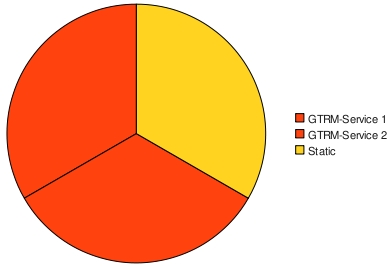
\includegraphics[width=0.7\textwidth]{piechart.jpeg}
  \caption{Pie chart for resource allocation.}
  \label{fig:Piechart}
\end{figure}

The slices in the pie chart of Figure~\ref{fig:Piechart} represent two
different sets of applications. The static yellow slice consists of
applications that are not managed by GTRM and share the resources
according to the predefined setting given by the slice. Applications
that belong to this set usually do not vary their resource requirement
or are hard real-time, which means they should be given enough resource
so that their deadlines are met. 

The red set shows two applications managed by the GTRM framework. These
application might implement the service level adaptation paradigm.
Applications belonging to this slice usually do vary their resource
requirements, or can change the quality of the computation to adapt to the
available resources. In Figure~\ref{fig:Piechart} there are two applications
(also called services) of this type.

All applications that are managed by the GTRM run as services under the 
GTRM-slice. A service can reserve a minimum percentage of allocated 
resources referring to its parent slice.
In the Pie chart above the static slice would be guaranteed a minimum of 
\sfrac{1}{3} of the total resources while the two GTRM services are given 

half of the \sfrac{2}{3} reserved by its parent slice, therefore obtaining
a minimum of \sfrac{1}{3} of the total available resources each.

In the GTRM slice, some of the applications are service level aware and some
other are not. Ideally all applications running in the GTRM-slice should, 
if it makes sense to the application, have a concept of service level.
Each application is assigned a weight, that sets how much responsibility
for the adaptation is taken care by the application that changes its service
level and how much adaptation should be realized via resource allocation.
All applications in the GTRM slice must implement the performance evaluatio
via matching function and the communication with the resource manager via
socket.

\subsection{Resource allocation in practice}
The resource split shown in Figure~\ref{fig:Piechart} is made by creating 
a \texttt{gtrm.slice} file in the folder \texttt{/etc/systemd/system}.
Any application that wants to take advantage of the GTRM capabilities needs
to create a service file in the same folder. When the service is started a folder named \texttt{gtrm.slice} will be created in the corresponding cgroup-controller-folder to represent the slice. The controller is a combination of the CPU-and CPUAccounting, \texttt{cpu,cpuacct}. The applications run in this slice will be represented as a folder within the slice-folder. The resulting path to the service will look like this.

\begin{verbatim}
/sys/fs/cgroup/cpu,cpuacct/gtrm.slice/gtrm.service/
\end{verbatim}

The unit file to represent the \texttt{gtrm.slice} is defined as follows. Here the only parameter specified is the amount of CPUShares. By setting this field the system is given the ability to change the CPUShares of this slice.
\subsubsection{gtrm.slice}
\begin{verbatim}
[Unit]
[Slice]
CPUShares=1024
\end{verbatim}

Any service file in the \texttt{/etc/systemd/system} folder overrides a service file for the same application declared somewhere else. The following describes the service files used by our test applications.

\subsubsection{gtrm-test.service and gtrm-test2.service}
\begin{verbatim}
[Unit]
[Service]
ExecStart=/mnt/flash/test-gtrm-app 50 10 0 0 0 0.1 0.5 0.04
CPUShares=100
Slice=gtrm.slice
\end{verbatim}

If no such file is created, by default, \texttt{systemd} defines a slice called \texttt{system.slice} located in \texttt{/usr/lib/systemd/system}. All services will belong to this slice unless another slice has been specified. 
\subsubsection{system.slice}
\begin{verbatim}
[Unit]
Description=System Slice
Documentation=man:systemd.special(7)
DefaultDependencies=no
Before=slices.target
Wants=-.slice
After=-.slice
\end{verbatim}

\texttt{DefaultDependencies} is set to \emph{no} to disable some non-essential 
dependencies. The \texttt{Before} and \texttt{After} fields makes sure that 
the units are started in the correct order, if necessary delaying one unit to 
make sure the other starts first. The unit(s) specified in the \texttt{Wants}-
field will start when this unit is started. In this case the \texttt{-.slice} 
will be started simultaneously as \texttt{system.slice}, but the 
\texttt{After} field ensures that \texttt{system.slice} will start-up first of 
them. This slice is given the default amount of CPUShares which is 1024, since 
nothing is specified in the unit file.

\section{Sequence Diagram}

The sequence diagram in Figure~\ref{fig:sdiag} describes the flow of 
execution of the system via pseudo-code. Some functions call that are 
not relevant and have been left out. 
\subsection{Application}
The application computes its performance (matching function), via a 
function called \texttt{calculate\_performance()}. According to its value,
and eventually to the performance multiplier received from the resource
manager at the past step, the service level of the application is adjusted by
calling \texttt{update\_service\_level()}. Finally, the resource manager
is notified via the \texttt{send\_performance()} call. 
Receiving the performance multiplier is done via a non-blocking socket which
means that the application does not have to wait for the resource manager to 
send it. If there are messages containing performance multipliers on the 
socket, only the newest value is used. If the socket is
empty the performance multiplier is set to one which corresponds to use of the 
update rule in Equation~\ref{eq:simple_sl_rec}.

\begin{figure}[t]
    \centering
    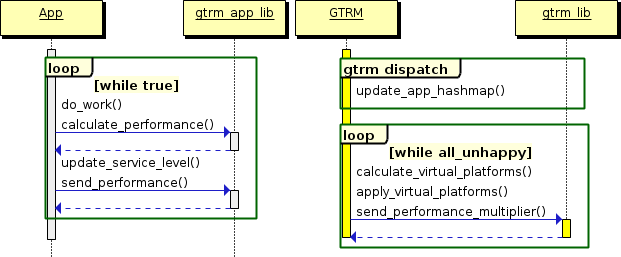
\includegraphics[width=0.9\textwidth]{diag.png}
    \caption{Sequence diagram}
    \label{fig:sdiag}
\end{figure}

\subsection{Resource manager, GTRM}
The resource manager consists of parallel parts. Upon receiving the
performance of an application, the handler (or dispatch function)
corresponding to the reception event is executed. In the sequence diagram of
Figure~\ref{fig:sdiag}, this call is labeled as \texttt{gtrm\_dispatch}.
Its main responsibility is to read and parse the received message and 
then update the hashmap containing the relevant data about the application
that sent the performance measurement. Meanwhile, the resource management 
runs as a part of the main resource manager loop. The resource management
algorithm uses the information in the hashmap to calculate the new virtual
platforms via the function \texttt{calculate\_virtual\_platforms} according
to Equation~\eqref{eq:RecursionForResources} and~\eqref{eq:RecursionForResources}.
These virtual platforms are then used to set the amount of CPUShares to
be given to each application in the call to \texttt{apply\_virtual\_platforms}.

To ease the service level adaptation, the resource manager also sends a
suggestion to the application, that depends on how much the virtual platform
is changed in the current round via a call to 
\texttt{send\_performance\_number}.

\chapter{Use cases}
\label{chp:usecases}

This chapter introduces relevant use cases that were the basis for the
work and guided the design of the system. In all the use cases it is assumed
that the resource available to the static slice is correctly sized, so that
the GTRM-slice does not have any more available than the allocated resource
and has to distribute it to the applications running within the slice.

\section{Nominal Conditions}

In nominal conditions, the system is well dimensioned. The applications
running inside the GTRM slice can be run at maximum service level without 
overloading the hardware.

The service level for all the running applications should be at the
highest possible value. The matching functions of the applications should
be either positive or zero for the applications and the deadlines of all
the running services should be hit.

\section{Overload Conditions (Streaming Dependant)}

In this second case, the streaming application is overloading the system.
The applications subsequently mentioned are all included in the GTRM slice,
that should allocate the resources available for them in order to match
the deadlines of every applications, including the streaming service.

The detailed conditions addressed are the following:
\section{Normal mode}
\begin{enumerate}
\item The camera is filming a scene that causes a high load. This may happen
  because the camera itself is moving around or because the scenary is
  very dynamic.
\item Service level aware applications are running together with the
  streaming service. These applications (including the streaming one) adapt
  their service level (and therefore the quality of their computation).
\item The GTRM increases the resource given to the applications with the
  worst performance (matching function). The resource is taken from other,
  better performing, applications on the same slice. These better performing
  services lower their service level to accomodate the change in the resource
  allocation.
\item The scene becomes more static or the camera stops, therefore inflicing
  a lighter load on the system. The service level of the applications can be
  increased since the streaming one is not so demanding in terms of resource.
\item The GTRM and SL adaptation will not drag down performance compared to the old system.
\end{enumerate}

The matching function of all the applications should be close to zero, since
they can all adjust their service level in a reasonable way during the
execution. The frame rate for the video streaming should be constant during
the execution, because the internal service adaptation of the streaming
service should take care of adjusting the compression level of the image.

\section{Overload Conditions (Non-Streaming Dependant)}

At the beginning of this use case the static slice is not fully loaded,
therefore some of the resource may be transfered from it to the GTRM
managed slice.

\begin{enumerate}
\item The static slice is not consuming all the resource allocated to it,
  therefore the GTRM slice can collect some of the remaining resource. The
  applications belonging to the GTRM slice can raise their service level to
  a value that is higher than the one that would be the equilibrium point
  in the nominal conditions.
\item The resource demand of the static slice starts to grow.
\item The service level of the applications belonging to the GTRM slice
  adapt, lowering the quality of the computation, until a new equilibrium
  is reached.
\item The demand of the static slice becomes lower again and the resource
  is released to the GTRM slice. The service level increase and the resource
  is redistributed to the applicaions on the GTRM slice.
\end{enumerate}

Again, the frame rate of the streaming application should be the same
during the execution. Also, the applications on the static slice should be
able to run without harm even when causing a higher (but still within the
amount of resource statically allocated) load onto the system.

\section{GTRM slice empty and filled}

This is a corner case, where no applications are running within the GTRM
slice. The static slice is allowed to use the entire amount of resource if
necessary. During the test case, some applications of the GTRM slice are
started and the virtual platforms should be adjusted accordingly, taking
resource from the static slice until the size of the static slice meets
the original allocation. If sized correctly, the matching functions of the
applications belonging to the GTRM slice should be zero or positive and
their service level should settle to an equilibrium value.

\section{Applications with different weights}

During this test, some applications are run in the GTRM slice. However, these
applications are highly heterogeneous --- which means that they have different
weights and they are willing to adjust their service level to various extents.
Some applications are eager to help the infrastructure and will lower their
requirement easily, while some other applications are more reluctant to
reduce the quality of the performed computation.

\begin{enumerate}
\item As a starting point, all the applications running in the GTRM slice
  have a positive or zero matching function, meaning that they are satisfied
  with the amount of resource assigned to them.
\item The performance of one of the application decreases, for example due to
  an increase in its computational load.
\item The GTRM and the service level adaptation starts trying to compensate
  for that.
\end{enumerate}


It is expected that the system reaches a stable point. The applications with
the higher weights adapt their matching function mainly due to an increase
in the amount of allocated resource. The allocation with lower weights cope
with the reduced resource availability by decreasing their service level.

\section{Nominal conditions in overload case}

In this case, a number of applications are running with reasonable
performance levels and no adaptation is needed. The system is subsequently
loaded to the point where some of the applications can not be satisfied.

\begin{enumerate}
\item A number of applications are running with good performances and 
  no service level adaptation or resource management is needed.
\item A new application is started with a default service level.
\item The resource manager takes care of allocating the resource to the
  new application, redistributing the available capacity. At the same
  time, the service level adjustment within the application tries to match
  the amount of resource given by the GTRM.
\item The amount of load introduced in the system is too much for the
  applications to be entirely satisfied. Some applications still have a 
  negative matching function, despite having reduced their service
  level to the minimum value.
\end{enumerate}

The system reaches a stable point where not all applications have a good
performance. The applications that supports the service level adaptation 
lowered their quality as much as possible. The GTRM loop will continue to
try to adjust to the current conditions.

\chapter{Experimental Results}
\label{chp:test}

% The end result will be a working prototype that can demonstrate that 
% the system works and what results that can be expected. These are the 
% main aspects that we want to test. To provide results and to prove that 
% the thesis is valid, thorough testing is required. The main focus of the 
% test is to see if the following can be achieved.
% \begin{itemize}
% \item Can we keep the FPS we want even during high load of the system.
% \item Can we adapt so that other applications can perform well during high loads as well. 
% \end{itemize}
% The test output consist of logs showing CPU-time for applications along 
% with their service levels, performance and virtual platforms. The CPU-time
% differ between how much resources are assigned to each application and how
% much is actually used and it is of interest to see how much they vary if 
% any. The FPS and video quality are other outputs that has to be taken into 
% the result.
% It is also desirable to test if the system can fulfill the 
% previously described use cases.
% \begin{itemize}
% \item The first and simplest case is a camera that is still and filming 
%   a scenery which does not change notably. Here it is expected maximal 
%   quality of the images since the scene itself does not require a lot 
%   of resources. 
% \item Next step is to test more complex scenery, for example scenery 
%   with a lot of different things going on at the same time. This will 
%   stress the video streaming and we want to make sure that if necessary 
%   the quality will be reduced in favor for a steady FPS.
% \item A moving PTZ-camera will cause a high load when it is moving 
%   around. This will cause the whole picture to be redrawn and not partly 
%   as when the image is still, and will be the ultimate stress test for 
%   the streaming part.
% \item By running different test applications that are resource demanding 
%   the camera can be tested during intense CPU-loads. Some of the 
%   applications will have a linear relationship between computational 
%   time and the SL while others will have a non linear one. This matters 
%   since the SL adaptation assumes a linear relationship between the SL 
%   and the computational time. If the steps in SL are small enough the 
%   linear relationship could still be assumed even for non linear ones.
% \end{itemize}

This chapter describes the tests that have been conducted on the entire
architecture to validate the claims. The tests will resemble the envisioned
use cases.

A first set of tests is obtained by starting and stopping different 
test-applications on the Axis P3367 camera. These applications run on 
the GTRM-slice and their resource is managed by the GTRM itself. The slices
and services are started and stopped with the command line tool 
\texttt{systemctl}~\cite{systemctl}.

As previously discussed, the resource available in the camera is split into
two different top slices. The first one is the system slice, that contains
all the normal services. The second one is the GTRM slice, that contains
applications that are possibly service level aware, the resource devoted to
which are managed by the GTRM. The command line tool \texttt{systemd-cgls}
shows the layout of the slice tree. Its output is shown in
Figures~\ref{fig:systemd-cgls2a} and \ref{fig:systemd-cgls2b}.
The system slice has been given $CPUShares = 1024$, while the GTRM slice got 
$CPUShares = 256$, meaning that the resource is split $\frac{4}{5}$ to 
$\frac{1}{5}$, between the two slices. 

\begin{figure}[h]
    \centering
    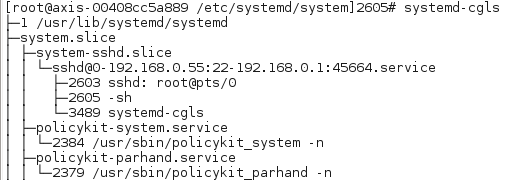
\includegraphics[width=0.8\textwidth]{systemd-cgls2}
    \caption{The first lines of the output from  systemd-cgls.}
    \label{fig:systemd-cgls2a}
\end{figure}

\begin{figure}[h]
    \centering
    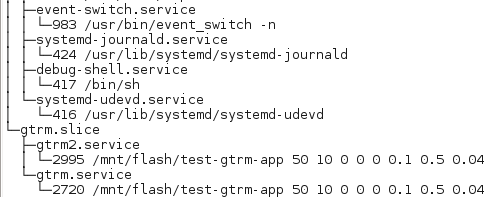
\includegraphics[width=0.8\textwidth]{systemd-cgls1}
    \caption{The last lines of the output from systemd-cgls.}
    \label{fig:systemd-cgls2b}
\end{figure}

To test the system, several test applications are run together, specifying
different parameters for each of them.%
When started, the test applications takes $10$ parameters, described in 
the box below. These parameters are modified in different tests. By 
varying the \texttt{weight} parameter from $0$ to $1$, the applications can 
be set somewhere between the extremes of only adapting through resource
allocation and only adapt through service level modification.
By varying the \texttt{a\_cpu} and \texttt{b\_cpu}, the emulated relationship
between service level and resource requirement is changed. While
\texttt{b\_cpu} represents service level independent load, \texttt{a\_cpu}
denotes the relationship between the set service level and the service level
dependent load that the application excerpt on the platform. The parameter
\texttt{epsilon} makes the service level adaptation slower or faster. All
services are given an initial $CPUShares = 100$, to be able to send their first message to \texttt{systemd} relatively fast.

\begin{framed}
\begin{flushleft}
	\textbf{\emph{test-gtrm-app.c(int argc, char* argv[])}} \newline
	The argv[] gets parsed to the following variables in the following 
  orders:
	\begin{itemize}
		\item float service\_level, Sets the starting value for the service 
      level.
		\item float a\_cpu, Used for calculating the cpu\_req.
		\item float b\_cpu, Used for calculating the cpu\_req.
		\item float a\_mem, Not used.
		\item float b\_mem, Not used.
		\item double epsilon, Affects how quickly the SL adapts.
		\item double weight, Determines how much of the adaptation that will 
      be made by the RM or by the SL adaptation. Is defined between 0 and 1.
		\item double deadline, The deadline for the job.
	\end{itemize}
	The cpu requirement is a linear function of the SL: 
  $cpu\_req = a\_cpu*ls +b\_cpu  $. Cpu\_req is simply the number 
  of calculations that will be performed each job. 
\end{flushleft}
\end{framed}	

In the tests, all the applications are launched at the same time. The
applications are expected to converge to a matching function close to or
equal to zero, with a service level that should stabilize over time. It is 
also expected that the resource manager initially assigns the same amount
of resource to all the applications. As their demands and adaptation
rates vary, the applications service level and virtual platforms does not 
have to converge identically, but if the system works as intended all the
applications should end up with a matching function close to zero.

The tests are performed by starting the services one by one. Every time 
an application is added, the system is expected to reset the virtual
platforms and assign to each application the same amount of resources. 
After that the system will then manage the resources and service level 
until all the applications are satisfied with their performance level.
Notice that the resource manager is managing only $90\%$ of the total 
shares assigned to it. This is a parameter of GTRM that could be changed
upon request, and the $10\%$ unused resource is intended as a slack, for
example to run the resource manager itself.

\subsection{Test 1: four applications with the same weights, 
  service level and resource adaptation}

\begin{figure}[th]
\centering
  \begin{minipage}{0.49\textwidth}
  \centering
  \includegraphics[width=\textwidth]{"tools/plot/logs/test1/vp"}
  \subcaption{Virtual Platforms}
  \end{minipage}
  \hfill
  \begin{minipage}{0.49\textwidth}
  \centering
  \includegraphics[width=\textwidth]{"tools/plot/logs/test1/sl"}
  \subcaption{Service Levels}
  \end{minipage}
  \begin{minipage}{0.49\textwidth}
  \centering
  \includegraphics[width=\textwidth]{"tools/plot/logs/test1/f"}
  \subcaption{Matching Functions}
  \end{minipage}
\caption{Results for Test 1.}
\label{fig:test1}
\end{figure}

In this test, four applications are started, one every 10 seconds. 
The applications are started with the settings shown in 
Table~\ref{tab:settings_test1}. The result is shown in 
Figure~\ref{fig:test1}. 

\begin{table}[h!]
  \centering
  \begin{tabular}{|c|c|c|c|c|c|c|}
  \hline 
   \emph{app} & $SL_{t=0}$ & \textbf{$a_{cpu}$} & 
   \textbf{$b_{cpu}$} & \textbf{$\epsilon$} & \emph{weight} & 
   \emph{Deadline} \\ \hline
  app1 & 75 & 10 & 0 & 0.06 & 0.5 &0.04  \\ \hline
  app2 & 75 & 20 & 0 & 0.06 & 0.5 &0.04  \\ \hline
  app3 & 75 & 10 & 0 & 0.01 & 0.5 &0.04  \\ \hline
  app4 & 75 & 10 & 0 & 0.01 & 0.5 &0.04  \\ \hline        
  \end{tabular}
  \caption{Settings for the test applications in Test 1.}
  \label{tab:settings_test1}
\end{table}

It can be seen that the applications receive different amount of resources
and settle to different service levels. Application 4, which is the last
one to enter the pool, starts with a very negative matching function. The
re-arrangement of resources allows the application to obtain a higher virtual
platform and therefore compute at a higher service level. It can also be
observed that --- despite the performance functions being quite noisy --- the
service levels settle to an equilibrium, as well as the virtual platforms.

\subsubsection{Comments on the results}
See the plots in figure \ref{fig:test1} and table \ref{tab:settings_test1}.
The plots behaves on the whole as expected from the settings in 
Table~\ref{tab:settings_test1}.
The mean of the noisy performance converges to zero which corresponds to each 
application finding a pairing of SL and virtual platform (VP). In the plot a 
higher/lower SL gives a higher/lower Virtual platform. The SL/VP combination
for app2 becomes different since the $a_{cpu}$ is twice that of the other apps 
resulting in a half as big SL compared to what it would have been otherwise. 
The VP resets after a new app has been started as it should. The SL for app 
3 and 4 converges slower than that of app 1 and 2 because of the lower
$\epsilon$ in app 3 and 4.

\subsection{Test 2: four applications with different weights, 
  service level and resource adaptation}

\begin{figure}[th]
\centering
  \begin{minipage}{0.49\textwidth}
  \centering
  \includegraphics[width=\textwidth]{"tools/plot/logs/test2/vp"}
  \subcaption{Virtual Platforms}
  \end{minipage}
  \hfill
  \begin{minipage}{0.49\textwidth}
  \centering
  \includegraphics[width=\textwidth]{"tools/plot/logs/test2/sl"}
  \subcaption{Service Levels}
  \end{minipage}
  \begin{minipage}{0.49\textwidth}
  \centering
  \includegraphics[width=\textwidth]{"tools/plot/logs/test2/f"}
  \subcaption{Matching Functions}
  \end{minipage}
\caption{Results for Test 2.}
\label{fig:test2}
\end{figure}

In this second test, four applications are started as done for the previous
one. The difference here is that these applications have different weights,
which indirectly governs how much of the adaptation that should be made by 
the application or by the GTRM. 
For a summary of the relevant data for the experiment, see 
Table~\ref{tab:settings_test2}.

\begin{table}[h!]
  \centering
  \begin{tabular}{|c|c|c|c|c|c|c|}
 	\hline 
   \emph{app} & $SL_{t=0}$ & \textbf{$a_{cpu}$} & 
   \textbf{$b_{cpu}$} & \textbf{$\epsilon$} & \emph{weight} & 
   \emph{Deadline} \\ \hline
	app1 & 75 & 10 & 0 & 0.06 & 0.2 &0.04  \\ \hline
	app2 & 75 & 20 & 0 & 0.06 & 0.4 &0.04  \\ \hline
	app3 & 75 & 10 & 0 & 0.01 & 0.6 &0.04  \\ \hline
	app4 & 75 & 10 & 0 & 0.01 & 0.8 &0.04  \\ \hline        
  \end{tabular}
  \caption{Settings for the test applications in Test 2.}
  \label{tab:settings_test2}
\end{table}

Figure~\ref{fig:test2} shows the results in terms of virtual platforms,
service levels and matching functions. As can be seen, the performance
functions, despite being noisy, converge to signals with zero mean.

\subsubsection{Comments on the result.} 
See the plots in figure \ref{fig:test2} and table \ref{tab:settings_test2}.
This test behaves alot like the previous one but with one difference in how 
the SL/VL combinations converge. The main point of this test is to see how the 
weight affects the VP:s convergence points.
As can be seen in the plot of the virtual platforms in fig \ref{fig:test2}, 
the applications with higher weights are assigned a higher VP which is in 
accordance with the theory.

\subsection{Test 3: four applications with zero weights and 
  service level adaptation}

In this third test, four applications are started as done for the previous
ones. However, the weights of the applications are set to zero. With all
weights set to zero the virtual platforms are not expected to change.
The result is shown in Figure~\ref{fig:test3}.

\begin{figure}[th]
\centering
  \begin{minipage}{0.49\textwidth}
  \centering
  \includegraphics[width=\textwidth]{"tools/plot/logs/test3/vp"}
  \subcaption{Virtual Platforms}
  \end{minipage}
  \hfill
  \begin{minipage}{0.49\textwidth}
  \centering
  \includegraphics[width=\textwidth]{"tools/plot/logs/test3/sl"}
  \subcaption{Service Levels}
  \end{minipage}
  \begin{minipage}{0.49\textwidth}
  \centering
  \includegraphics[width=\textwidth]{"tools/plot/logs/test3/f"}
  \subcaption{Matching Functions}
  \end{minipage}
\caption{Results for Test 3.}
\label{fig:test3}
\end{figure}

\subsubsection{Comments on the results}
See the plots in fig \ref{fig:test3}
As expected there is no change in VP except for the even split when a new application is added. The Performance looks a bit noisier than previously indicating an improvement when both SL and VP adaptation is being used.

\subsection{Test 4: four applications with weights equal to one and 
  service level adaptation}

This test is the dual of the previous one but all the weights are set to 1.
With all weights set to one the adaptation is expected to be done by varying the virtual platforms. The result is shown in Figure~\ref{fig:test4}. 

\begin{figure}[th]
\centering
  \begin{minipage}{0.49\textwidth}
  \centering
  \includegraphics[width=\textwidth]{"tools/plot/logs/test4/vp"}
  \subcaption{Virtual Platforms}
  \end{minipage}
  \hfill
  \begin{minipage}{0.49\textwidth}
  \centering
  \includegraphics[width=\textwidth]{"tools/plot/logs/test4/sl"}
  \subcaption{Service Levels}
  \end{minipage}
  \begin{minipage}{0.49\textwidth}
  \centering
  \includegraphics[width=\textwidth]{"tools/plot/logs/test4/f"}
  \subcaption{Matching Functions}
  \end{minipage}
\caption{Results for Test 4.}
\label{fig:test4}
\end{figure}

\clearpage
\subsubsection{Comments on the results}
See the plots in figure \ref{fig:test4}
From comparing the two SL plots from test1 ,in figure \ref{fig:test1},and test4, in figure \ref{fig:test4}, it seems like the SL for app3 and app4 converges slower in the test 4 case. 
The VP plot also displays greater difference between the 4 applications than in the test 1 case. Although these changes are small in comparison to the changes in test 3 it can be argued that more of the adaptation is done by varying the VP in test 4 as opposed to in test 1.
Once again the performance seems a bit noisier compared to the test 1 case indicating an improvement when both SL and VP adaptation is being used.

\subsection{Test 5: four applications with no service level adaptation}

Four applications are started one by one with the settings in 
Table \ref{tab:settings_test5}. As can be seen, the value of $a\_cpu$ is
zero for all the applications, meaning that the service level is not
at all affecting the amount of resources requested on the application side.
According to proposition 3.2 in ``A Game-Theoretic Resource Manager for 
RT Applications''~\cite{gtrm}, the normalized virtual platforms will tend 
to the values given by
\begin{equation}
  \tv_i^* \to \frac{\lambda_i}{\sum_{j=1}^{n}\lambda_j},
  \label{eq:SpecialStationaryPoint}
\end{equation}

\begin{table}[h]
  \centering
  \begin{tabular}{|c|c|c|c|c|c|c|}
  \hline 
   \emph{app} & $SL_{t=0}$ & \textbf{$a_{cpu}$} & 
   \textbf{$b_{cpu}$} & \textbf{$\epsilon$} & 
   \emph{weight} & \emph{Deadline} \\ \hline
  app1 & 75 & 0 & 10 & 0.06 & 0.2 &0.04  \\ \hline
  app2 & 75 & 0 & 10 & 0.06 & 0.4 &0.04  \\ \hline
  app3 & 75 & 0 & 10 & 0.01 & 0.6 &0.04  \\ \hline
  app4 & 75 & 0 & 10 & 0.01 & 0.8 &0.04  \\ \hline        
  \end{tabular}
  \caption{Settings for the test applications in Test 5.}
  \label{tab:settings_test5}
\end{table}

\begin{figure}[th]
\centering
  \begin{minipage}{0.49\textwidth}
  \centering
  \includegraphics[width=\textwidth]{"tools/plot/logs/test5/vp"}
  \subcaption{Virtual Platforms}
  \end{minipage}
  \hfill
  \begin{minipage}{0.49\textwidth}
  \centering
  \includegraphics[width=\textwidth]{"tools/plot/logs/test5/f"}
  \subcaption{Matching Functions}
  \end{minipage}
\caption{Results for Test 5.}
\label{fig:test5}
\end{figure}

Figure~\ref{fig:test5} shows the convergence of the virtual platforms
and the corresponding matching functions. As can be seen, the matching
functions of all the applications become positive, meaning that the
architecture is capable of handling the load produced by the applications
correctly, despite the reduction in the virtual platforms.

Also, as can be seen, all the virtual platforms converge to the same value,
except for the one given to the last application, that is the last 
(since it started later) to reach a positive matching function. 
All the resources that are not distributed are therefore given to this
application to help it recover faster. When the matching functions are
positive, the allocation of resource stays unchanged, since there is no need
for redistribution.

\begin{table}[h]
  \centering
  \begin{tabular}{|c|c|c|c|c|c|c|}
  \hline 
   \emph{app} & $SL_{t=0}$ & \textbf{$a_{cpu}$} & \textbf{$b_{cpu}$} & \textbf{$\epsilon$} & \emph{weight} & \emph{Deadline} \\ \hline
  app1 & 75 & 0 & 120 & 0.06 & 0.2 &0.04  \\ \hline
  app2 & 75 & 0 & 120 & 0.06 & 0.4 &0.04  \\ \hline
  app3 & 75 & 0 & 120 & 0.01 & 0.6 &0.04  \\ \hline
  app4 & 75 & 0 & 120 & 0.01 & 0.8 &0.04  \\ \hline        
  \end{tabular}
  \caption{Settings for the test applications in Test 5
    with a higher $b\_cpu$ value.}
  \label{tab:settings_test5b}
\end{table}

\begin{figure}[tb]
\centering
  \begin{minipage}{0.49\textwidth}
  \centering
  \includegraphics[width=\textwidth]{"tools/plot/logs/test5b/vp"}
  \subcaption{Virtual Platforms}
  \end{minipage}
  \hfill
  \begin{minipage}{0.49\textwidth}
  \centering
  \includegraphics[width=\textwidth]{"tools/plot/logs/test5b/f"}
  \subcaption{Matching Functions}
  \end{minipage}
\caption{Results for Test 5 with a higher $b\_cpu$.}
\label{fig:test5b}
\end{figure}

\newpage
\subsubsection{Comments on the results}

\begin{flushleft}
\emph{Test with a lower $b_{cpu},$}
\end{flushleft}
See the plots in figure \ref{fig:test5} and table \ref{tab:settings_test5}.
In this test only the VP and performance plots are of interest since $a_{cpu}=0$ and hence changes in SL has no effect.
The VP for the different applications does not seem to converge to the theoretical ones which probably is because of a too small static SL, $b_{cpu}$.
The effects of this small $b_{cpu}$ can be seen in the performance plot in figure \ref{fig:test5} when 25 < t35 where the performance is stuck in the upper half plane indicating that the applications need a higher SL 
in order to make use of all of their available CPU. After time t = 45 the time between updates of the performance in the RM increases drastically, (the performance plots shows the performance that the RM has received). This is most likely due to a temporary problem with sending messages on DBus which in turn might have been caused by the flood of sent messages due to the high performance.

The test is repeated, increasing the value of $b_{cpu}$. Also, in this
second case, a resource hungry application is started on the system slice 
in an attempt to limit the noise in performance. The settings for the
test can be seen in Table~\ref{tab:settings_test5b} while 
Figure~\ref{fig:test5b} shows the matching functions and the virtual
platforms in this second case.



\begin{flushleft}
\emph{Test with a higher $b_{cpu}$,}
\end{flushleft}
See the plots in figure \ref{fig:test5b} and table \ref{tab:settings_test5b}.
The values that the VP for the different applications converges to, compensated for the scale factor,  together with the theoretical values and the weights are shown in table \ref{tab:VP_test5b}.
From the table it can be seen that the applications have not reached their theoretical values, however they are not far from them.
The discrepancy might be explained by all the noise that performance still displays. This noise seems to have been reduced by the cpu hog on the system.slice.



\subsection{Test 6: mixed load of applications with and without service 
  level adaptation}


In this last test, five applications are started one by one with the 
settings shown in Table~\ref{tab:settings_test6}. Figure~\ref{fig:test6}
depicts the result of the run.

\begin{table}[h]
  \centering
  \begin{tabular}{|c|c|c|c|c|c|c|}
  \hline 
   \emph{app} & $SL_{t=0}$ & \textbf{$a_{cpu}$} & 
   \textbf{$b_{cpu}$} & \textbf{$\epsilon$} & 
   \emph{weight} & \emph{Deadline} \\ \hline
  app1 & 50 & 0  & 30 & -     & 0.5 &0.04  \\ \hline
  app2 & 50 & 20 & 0  & 0.01  & 0.5 &0.04  \\ \hline
  app3 & 50 & 0  & 30 & -     & 0.2 &0.04  \\ \hline
  app4 & 50 & 20 & 0  & 0.01  & 0.2 &0.04  \\ \hline
  app5 & 50 & 10 & 0  & 0.002 & 0.8 &0.04  \\ \hline                
  \end{tabular}
  \caption{Settings for the test applications in Test 6}
  \label{tab:settings_test6}
\end{table}

\begin{figure}[th]
\centering
  \begin{minipage}{0.49\textwidth}
  \centering
  \includegraphics[width=\textwidth]{"tools/plot/logs/test6/vp"}
  \subcaption{Virtual Platforms}
  \end{minipage}
  \hfill
  \begin{minipage}{0.49\textwidth}
  \centering
  \includegraphics[width=\textwidth]{"tools/plot/logs/test6/sl"}
  \subcaption{Service Levels}
  \end{minipage}
  \begin{minipage}{0.49\textwidth}
  \centering
  \includegraphics[width=\textwidth]{"tools/plot/logs/test6/f"}
  \subcaption{Matching Functions}
  \end{minipage}
\caption{Results for Test 6.}
\label{fig:test6}
\end{figure}


\subsubsection{Comments on the results}
See the plots in Figure \ref{fig:test6} and Table \ref{tab:settings_test6}.
The plots looks as expected. That the weights influence how much VP an
application gets can be seen in that $VP_{app5}>VP_{app2}>VP_{app4}$. 
The small $\epsilon$ for app 5 makes the SL adaptation very slow.


\begin{table}[h]
  \centering
  \begin{tabular}{|c|c|c|c|}
 	\hline 
   \emph{app} & \emph{weight} & $VP_{theoretical}$ & $VP_{plot}$  \\ \hline
	app1 & 0.2 & 0.1 & 	0.17	\\ \hline
	app2 & 0.4 & 0.2 & 	0.23 \\ \hline
	app3 & 0.6 & 0.3 & 	0.28 \\ \hline
	app4 & 0.8 & 0.4 &  0.32 \\ \hline
  \end{tabular}
  \caption{Table showing the convergence of VP and weights in test 5b}
  \label{tab:VP_test5b}
\end{table}
\begin{comment}
\end{comment}

\section{Result discussion}

Overall the plots of the virtual platforms and the service level look good,
with the exception of the extremely noisy matching functions. They do 
however have zero mean which is why it is deemed as a good enough result.
There are a couple of possible explanations for the noisy performance; one
being the extra CPU that the GTRM slice receives when the system slice has
spare resources to lend. This introduces a disturbance driving the 
performance up. However when loading the system slice with a cpu hunger
application, no major changes in performance were shown.
To reduce the amount of noise in the matching functions, one could average
over a larger interval of samples, therefore smoothening the function's
behavior.

\chapter{Discussion, Conclusion and Future Work}
\label{chp:conclusion}

This thesis implemented a Game Theoretic Resource Manager (GTRM) on Axis
cameras, to distribute the CPU among multiple running applications that can
be adaptive in nature and vary their service level and the required
computation, together with the quality of the offered service.


\section{Result discussion}

Overall the plots of the virtual platforms and the service level looks good but the main problem are
the extremely noisy performances. They do however have zero mean which is why it is deemed as a good enough result.
There are a couple of possible explanations for the noisy performance ; one being the extra CPU that the gtrm slice receives when the system.slice has
spare resources to lend. This introduces a disturbance driving the performance up. However when loading the system.slice with a cpu hog no major changes in performance were shown.
Another explanation could be the delay in the sockets communication since delays tend to make systems oscillate. 
A third reason is simply a bug somewhere in the code.
The time between actions from the GTRM is irregular, how this affects the system has not been taken in to consideration.

\section{Conclusion}

The provided implementation demonstrated that the GTRM can be integrated into
\texttt{systemd} and run in an Axis camera. To this end, many steps have been
followed. First of all the Inter-Process Communication of the original GTRM
was succesfully converted from shared memory to socket communication. The
conversion was necessary to realize the integration with the camera
framework. The implementation of the socket-based IPC resembled the
code of the ``Notify'' feature, already included in the operating system.
However, the resulting code was harder to understand and debug, compared to
code completely written from scratch. The final result worked well and was
well integrated into \texttt{systemd}.

The transition from shared memory to socket usage also required a new data
structure for the applications. A hashmap was a natural choice. The
applications PIDs were the natural choice to be used for the hashmap keys.
The constant time-complexity of the data access provided by a hashmap does not
negatively impact on the GTRM performance. The provided implementation also
included macros for iterating through the hashmap, together with all the
normal functions for adding and retrieving elements. 

The resource management loop was inserted into the main loop of 
\texttt{systemd} and performed as expected. By changing to CPU-shares from
\texttt{cpu.quota} and \texttt{cpu.period}, the risk of causing a kernel 
panic by assigning more resource than available was eliminated. Since the
assignment of CPU-shares is done inside \texttt{systemd}, without the need of
communication over DBus, it does not require a significant amount of time.



\section{Future work}

The work done in this thesis should be extended completing the implementation
of a service level aware video streaming application. The performance of
the system can be further improved when more applications are using the
service level framework, therefore every application that can be ported to
the idea of service levels and varying quality should be improved.
Implementing the matching function calculation and the service level
adaptation would be the ultimate solution to the resource management and
prioritization problem. This would also eliminate the need for the static
cgroup slice, since all the applications would be running in the same slice,
managed by the GTRM.

The system itself is in need of further testing to track down bugs and
memory leaks, if any. Future work would consist of taking this rough
prototype and develop a more refined product. The consequences of the irregular update times of the VP
in the GTRM should be further looked into, there are simple solutions to using the longest time 
between updates for all updates which would give uniform updating to the cost of a slower controller.


This project is well 
integrated into Axis' version control and could easily be applied as a 
patch to future products. Also, it could be of interest to share this 
work with the \texttt{systemd} open source community.


\bibliographystyle{plain}
\bibliography{mybib}

\appendix

\chapter{Source Code Overview}

In this section follows an overview of the header and source files used in the system and their attributes.

\section{gtrm\_lib.c/h}
A library which contains various functions used by the resource manager to make various computations and inter process communication.

\subsection{struct rm\_app\_t}
Represents an application being managed and consists of the following fields.
\begin{itemize}
\item tid: Applications PID.
\item vp: Virtual platform.
\item vp\_old: Previous virtual platform.
\item performance: Performance, or matching function of the application.
\item weight: The current "weight" of the application.
\item happy: Indicates if the application is happy with its 

      current performance. This field was added to prevent application from sending their performance even when they are satisfied and nothing should be needed from the resource manager, eliminating unnecessary computations.
\item sa: Socket Address, used to send back the performance multiplier.
\end{itemize}

\subsection{struct gtrm\_t}
Stores various parameters used by the GTRM.
\begin{itemize}
\item c1: Constant used for computing epsilon, determines how much we will change the virtual platform.
\item c2: Another constant used for computing epsilon similar as c1.
\item iterations: Keeps track of how many iterations the GTRM has run.
\item all\_happy: Used to indicate if we have to make any adjustments to the resource allocations.
\item num\_apps: Total amount of applications that we are managing.
\item prev\_apps: The amount of applications in the previous iteration.
\end{itemize}

\subsection{void gtrm\_char2gtrmstruct(char* str, rm\_app\_t *re)}
Extracts data from a received string and store it as a struct instead. The data sent from an application consists of the PID, performance, weight and if the application is satisfied or not.
\begin{itemize} 
\item str: String to extract data from.
\item re: Struct to hold the extracted data.
\item Return value: None, the result is stored in \emph{re}.
\end{itemize}

\subsection{int gtrm\_send\_performance\_multiplier(double pm, int fd, struct sockaddr *sa)}
Sends a performance multiplier to an application via sockets.
\begin{itemize} 
\item pm: Performance multiplier to send.
\item fd: File descriptor used to send the performance multiplier.
\item sa: Socket address.
\item Return value: Always zero.
\end{itemize}

\subsection{double gtrm\_get\_epsilon(unsigned int iterations, unsigned int offset, double c1, double c2)}
Calculates the constant epsilon used by the resource manager.
\begin{itemize} 
\item iterations: Number of iterations run by the RM.
\item offset: If one, resets the time used in the iteration. This restarts the calculation.
\item c1: Constant, previously described.
\item c2: Constant, also previously described.
\item Return value: The calculated epsilon or one if this is the first iteration.
\end{itemize}

\subsection{void gtrm\_update\_performance\_multipliers(int gtrm\_fd, Hashmap *gtrm\_apps)}
Calculates, updates and sends the performance multiplier to each application, using the performance, virtual platform and the previous virtual platform for each application.
\begin{itemize} 
\item gtrm\_fd: File descriptor used to send the performance multiplier.
\item gtrm\_apps: Hash-map containing rm\_app\_t structs for each application.
\item Return value: None.
\end{itemize}

\subsection{void gtrm\_write\_log(Hashmap *gtrm\_apps, unsigned int num\_applications)}
Writes information about the resource management to a log file, which can then be used to generate some nice graphs.
\begin{itemize} 
\item gtrm\_apps: Hash-map containing rm\_app\_t structs for each application.
\item num\_applications: Used to make sure we don't try to print an empty hash-map.
\item Return value: None.
\end{itemize}

\section{manager.c/h}
One of the main files in systemd and is for example responsible for inter process communication. The following fields are added to the \emph{Manager} struct in manager.h:
\begin{itemize}
\item gtrm\_socket: String that represent the socket used by GTRM.
\item gtrm\_fd: A file descriptor, which is an integer, for communicating with GTRM.
\item gtrm\_event\_source: Used to determine the source of an event and how this event is supposed to be handled.
\item gtrm\_apps: Hash-map containing all the applications being managed by the GTRM.
\end{itemize}

\subsection{static int manager\_dispatch\_gtrm\_fd(sd\_event\_source *source, int fd, unit32\_t revents, void *userdata)}
Called when we receive the performance of an application.
\begin{itemize}
\item source: source of the event.
\item fd: file descriptor to the event source.
\item revents: Set by the kernel to indicate what event on the file descriptor that triggered the call to this function. In our case it is always the incoming event.
\item userdata: In this case it contains a reference to the manager.
\item Return value: Not used, always zero.
\end{itemize}

\subsection{static int manager\_setup\_gtrm(Manager *m)}
Used to setup the socket, event source and file descriptor for the resource manager. Called from manager\_startup and manager\_reload.
\begin{itemize}
\item m: Reference to the manager.
\item Return value: Zero if function ran correctly, otherwise it is set to the corresponding error number.
\end{itemize}

\subsection{int gtrm\_compute\_virtual\_platforms(Hashmap *apps, gtrm\_t *gtrm\_t)}
Calculates the amount of resources (virtual platform) for an application.
\begin{itemize}
\item apps: The hash-map containing information about the applications being managed.
\item gtrm\_t: Struct with parameters used when calculating the virtual platforms.
\item Return value: Not used, always zero.
\end{itemize}

\subsection{void gtrm\_apply\_virtual\_platforms(Manager* m)}
Computes and applies the amount of CPUShares that each application shall be given.
\begin{itemize}
\item m: Reference to manager, used to get the applications
\item Return value: None.
\end{itemize}

\subsection{int manager\_loop(Manager *m)}
The main loop of the system which continuously calls gtrm\_compute\_virtual\_platforms, gtrm\_apply\_virtual\_platforms and gtrm\_update\_performance\_multipliers if all applications are not satisfied with their performance.
\begin{itemize}
\item m: Reference to manager, used to get the applications.
\item Return value: Exit code of systemd.
\end{itemize}

\subsection{int manager\_set\_cpu\_shares(Manager *m, pid\_t pid, int shares)}
Sets the CPUShares of an application.
\begin{itemize}
\item m: Reference to manager, used to get the applications.
\item pid: Process identifier of the application.
\item shares: Amount of shares we want to set.
\item Return value: Zero if successful, one otherwise.
\end{itemize}

\section{gtrm\_app\_lib.c/h}
These files are used by the applications to get performance, send performance and setup IPC, for example.
In the header file the following structs are defined:
\subsection{struct \_job\_h}
A struct used to represent a job. Applications can have different type of jobs with different deadlines. We only use one type however.
\begin{itemize}
\item id: Identifier to keep track of a job being executed.
\item type: What type of job this is.
\item start\_timestamp: Time when the job was started.
\item end\_timestamp: Time when we were finished with job. The timestamps are used to calculate the total execution time of a job.
\end{itemize}

\subsection{struct \_application\_h}
Each application stores the relevant information in terms of resource management and SL-adaptation in this struct.
\begin{itemize}
\item application\_id: Identifier for an application.
\item jobs: Number of possible job types
\item weight: Determines how to divide the adaptation between the resource manager and service level adaptation.
\item performance\_multiplier: Depends on how the virtual platform has changed and is used for better service level adaptation.
\item total\_jobs: How many jobs that has been launched in total.
\item progress\_jobs: Jobs in progress.
\item completed\_jobs: Total amount of completed jobs.
\item expected\_response\_times: Array of the expected response time for each job type.
\item happy: Indicates if the application is satisfied with its performance or not.
\end{itemize}

\subsection{int gtrm\_lib\_setup\_socket(char* filename)}
Sets up a socket to communicate with the resource manager.
\begin{itemize}
\item filename: The socket needs a file to work, the parameter specifies its path.
\item Return value: Zero, not used.
\end{itemize}

\subsection{void gtrm\_lib\_send\_performance(\_application\_h *h, double performance)}
Sends the performance of an application to the GTRM.
\begin{itemize}
\item h: Struct representing an application.
\item performance: Performance or matching function to send to the GTRM.
\item Return value: None.
\end{itemize}

\subsection{int gtrm\_lib\_set(\_application\_h* a, uint types, uint64\_t* ert)}
Initializes the application struct with job types and their expected response times.
\begin{itemize}
\item a: Struct representing an application.
\item types: Number of different job types.
\item ert: Array of expected response time for each job type.
\item Return value: Exit status of function.
\end{itemize}

\subsection{static int manager\_setup\_gtrm(Manager *m)}
Used to setup the socket, event source and file descriptor for the resource manager. Called from manager\_startup and manager\_reload.
\begin{itemize}
\item m: Reference to the manager.
\item Return value: Zero if function ran correctly, otherwise it is set to the corresponding error number.
\end{itemize}

\subsection{double gtrm\_lib\_get\_performance\_number(\_application\_h* a, int job\_type)}
Calculates the peformance (matching function) by averaging the performance of the last ten jobs of a specified type.
\begin{itemize}
\item a: Struct representing an application.
\item type: Which job type for which we want to calculate the performance.
\item Return value: Applications performance.
\end{itemize}

\subsection{int gtrm\_lib\_update\_performance\_multiplier(\_application\_h *a)}
Receives the performance multiplier computed by the RM.
\begin{itemize}
\item a: Struct for representing the application, and storing the performance multiplier.
\item Return value: Zero, never used.
\end{itemize}

\subsection{int gtrm\_lib\_signalstart(\_application\_h* a, uint type)}
Indicates the start of a job.
\begin{itemize}
\item a: Struct for representing the application.

\item type: Type of the job that is started.
\item Return value: Identifier of the started job.
\end{itemize}

\subsection{int gtrm\_lib\_signalend(\_application\_h* a, uint id)}
Indicates the end of a job.
\begin{itemize}
\item a: Struct for representing the application.
\item Return value: Exit status.
\end{itemize}

\section{sl\_adapt.c}
Used by the streaming application, \emph{monolith}, to incorporate service level features.
\subsection{void setup\_sl\_adapt(float service\_level, double epsilon, double weight, double deadline\_seconds)}
Sets up deadline for computing the matching function and sets up the IPC with the resource management.
\begin{itemize}
\item service\_level: Initial service level.
\item epsilon: Constant which specifies service level adaptation rate.
\item weight: Determines how the much of the adaptation will be done by altering the service level or the changing the amount of resources.
\item deadline\_seconds: This deadline will correspond to the desired frame rate.
\item Return value: None.
\end{itemize}

\subsection{void sl\_adapt()}
Performs the service level adaptation, notifies the resource manager and writes some logging.
\begin{itemize}
\item Return value: None.
\end{itemize}


\subsection{test-gtrm-app.c(int argc, char* argv[])}
The argv[] gets parsed to the following variables:
\begin{itemize}
		\item float service\_level, Sets the starting value for the service level.
		\item float a\_cpu, Used for calculating the cpu\_req.
		\item float b\_cpu, Used for calculating the cpu\_req.
		\item float a\_mem, Not used.
		\item float b\_mem, Not used.
		\item double epsilon, Affects how quickly the SL adapts.
		\item double weight, Determines how much of the adaptation that will be made by the RM or by the SL adaptation.
		\item double deadline, The deadline for the job.

\end{itemize}
The cpu requirement is a linear function of the SL: $cpu\_req = a\_cpu*ls +b\_cpu  $. Cpu\_req is simply the number of calculations 
that will be performed each job. 





\end{document}
